% !TEX program = xelatex
\documentclass[12pt,a4paper]{report}

\usepackage{fontspec}
\setmainfont{Times New Roman}

\usepackage[top=2.5cm, bottom=2.5cm, left=3.0cm, right=2.0cm]{geometry}
\usepackage{amsmath,amssymb,amsfonts}
\usepackage{graphicx}
\usepackage[table]{xcolor}
\usepackage{colortbl}
\usepackage{booktabs}
\usepackage{tabularx}
\usepackage{array}
\usepackage{multirow}
\usepackage{longtable}
\usepackage{titlesec}
\usepackage{fancyhdr}
\usepackage{listings}
\usepackage[most]{tcolorbox}
\usepackage{hyperref}
\usepackage{caption}
\usepackage{subcaption}
\usepackage{float}
\usepackage{enumitem}
\usepackage{microtype}

% Định nghĩa màu sắc nhận diện
\definecolor{bkblue}{RGB}{0, 51, 153}
\definecolor{darkblue}{RGB}{0, 32, 96}
\definecolor{codebg}{RGB}{245, 247, 250}
\definecolor{framegray}{RGB}{210, 215, 225}
\definecolor{noteorange}{RGB}{217, 83, 30}
\definecolor{successgreen}{RGB}{34, 139, 34}

% Thiết lập liên kết hyperref
\hypersetup{
    colorlinks=true,
    linkcolor=bkblue,
    citecolor=bkblue,
    urlcolor=bkblue,
    bookmarksnumbered=true
}

% Cấu hình listings cho SPICE code
\lstset{
    backgroundcolor=\color{codebg},
    basicstyle=\ttfamily\small,
    breaklines=true,
    captionpos=b,
    frame=single,
    rulecolor=\color{framegray},
    keywordstyle=\color{bkblue}\bfseries,
    commentstyle=\color{gray}\itshape,
    stringstyle=\color{noteorange},
    numbers=left,
    numberstyle=\tiny\color{gray},
    stepnumber=1,
    numbersep=8pt,
    tabsize=2,
    showstringspaces=false
}

% Header và Footer
\pagestyle{fancy}
\fancyhf{}
\setlength{\headheight}{15pt}
\rhead{\small\textcolor{gray}{CO2037 - Báo Cáo Dự Án 3: LTspice Migration}}
\lhead{\small\textcolor{gray}{Trường ĐH Bách Khoa - ĐHQG-HCM}}
\rfoot{\small\thepage}
\lfoot{\small\textit{Nhóm 9 - Lớp Linh Kiện và Mạch Điện Tử}}
\renewcommand{\headrulewidth}{0.5pt}
\renewcommand{\footrulewidth}{0.5pt}

% Định dạng tiêu đề chương, mục
\titleformat{\chapter}[display]
  {\normalfont\bfseries\color{bkblue}}
  {\filleft\large\MakeUppercase{\chaptertitlename} \Huge\thechapter}
  {1ex}
  {\titlerule\vspace{1ex}\LARGE\filright}
  [\vspace{1ex}\titlerule]

\titleformat{\section}
  {\normalfont\Large\bfseries\color{bkblue}}{\thesection}{1em}{}
\titleformat{\subsection}
  {\normalfont\large\bfseries\color{darkblue}}{\thesubsection}{1em}{}
\titleformat{\subsubsection}
  {\normalfont\normalsize\bfseries}{\thesubsubsection}{1em}{}

\titlespacing*{\chapter}{0pt}{-10pt}{20pt}
\titlespacing*{\section}{0pt}{15pt}{8pt}
\titlespacing*{\subsection}{0pt}{10pt}{5pt}

\setlength{\parindent}{0pt}
\setlength{\parskip}{6pt}

\begin{document}

% =========================================================================
% TRANG BÌA
% =========================================================================
\begin{titlepage}
    \begin{center}
        \textbf{\large ĐẠI HỌC QUỐC GIA THÀNH PHỐ HỒ CHÍ MINH}\\
        \textbf{\large TRƯỜNG ĐẠI HỌC BÁCH KHOA}\\
        \textbf{\large KHOA KHOA HỌC VÀ KỸ THUẬT MÁY TÍNH}\\[1.5cm]

        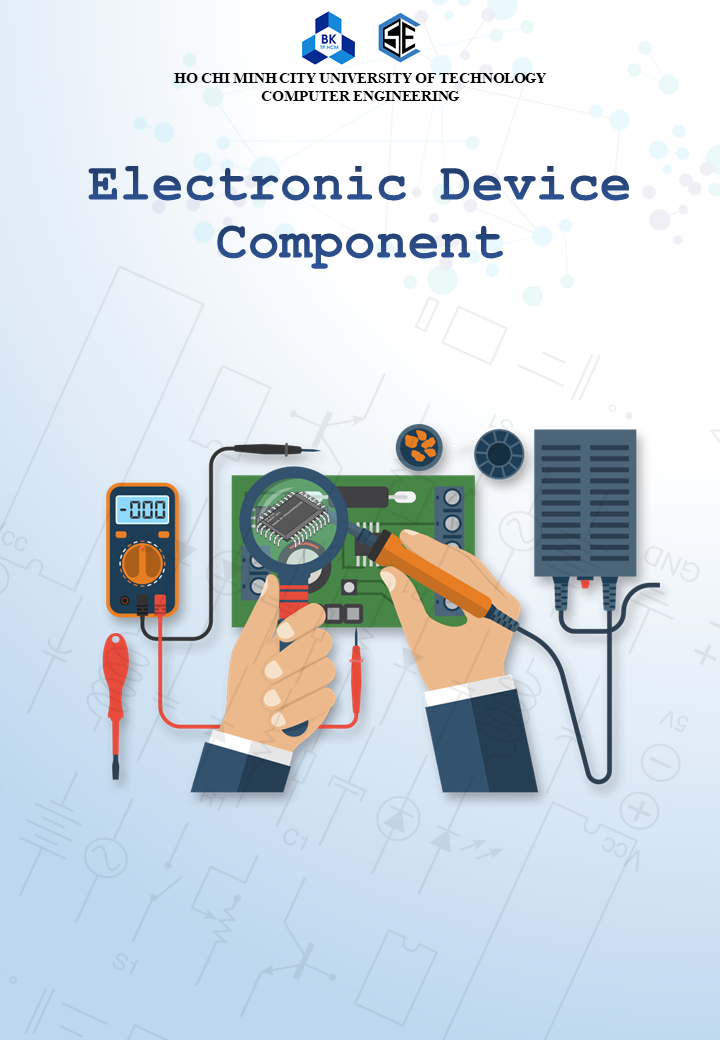
\includegraphics[width=3.2cm]{source/picture/cover.png}\\[1.5cm]

        \textbf{\Large BÁO CÁO BÀI TẬP LỚN -- DỰ ÁN 3}\\[0.3cm]
        \textbf{\LARGE\color{bkblue} XÂY DỰNG TÀI LIỆU THỰC HÀNH MỚI VỚI LTSPICE}\\[0.2cm]
        \textbf{\large Chuyển đổi 6 bài thực hành mô phỏng từ PSpice for TI sang LTspice}\\[1.5cm]

        \textbf{\large Môn học: LINH KIỆN VÀ MẠCH ĐIỆN TỬ (CO2037)}\\
        \textbf{\normalsize Học kỳ: HK251 (Năm học 2026--2027)}\\[2.0cm]

        \begin{flushleft}
            \begin{tabular}{ll}
                \textbf{Giảng viên hướng dẫn:} & TS. Lê Trọng Nhân \\
                \textbf{Lớp:} & L01 -- Nhóm: 9 \\
                \textbf{Sinh viên thực hiện:} & \\
                \quad 1. Phạm Đỗ Hồng Phúc & MSSV: 2510359 \\
                \quad 2. Lê Lương Vỹ & MSSV: 2214056 \\
                \quad 3. Nguyễn Bảo Duy Thành & MSSV: 2510372 \\
            \end{tabular}
        \end{flushleft}

        \vfill
        \textbf{\large Thành phố Hồ Chí Minh, Tháng 11/2026}
    \end{center}
\end{titlepage}

% =========================================================================
% THÔNG TIN DỰ ÁN VÀ BẢNG 5
% =========================================================================
\pagenumbering{roman}
\tableofcontents
\newpage
\listoftables
\newpage
\listoffigures
\newpage

\pagenumbering{arabic}

\chapter*{Thông Tin Dự Án và Nhóm Thực Hiện}
\addcontentsline{toc}{chapter}{Thông Tin Dự Án và Nhóm Thực Hiện}

Dự án 3 của học phần Linh kiện và Mạch điện tử (CO2037) hướng tới mục tiêu then chốt: Chuyển đổi toàn diện hệ thống 6 bài thực hành mô phỏng từ phần mềm độc quyền \textit{PSpice for TI} sang công cụ mã nguồn mở công nghiệp \textit{LTspice} (Analog Devices). Sản phẩm chuyển giao bao gồm bộ tài liệu hướng dẫn thực hành hoàn chỉnh mới, giải pháp đóng gói offline cho hệ thống phòng thí nghiệm cách ly mạng, bộ file thiết kế mô phỏng (.asc), và tài liệu giải đáp chi tiết dành cho giảng viên.

\vspace{0.5cm}
\begin{table}[H]
\centering
\caption{Thông tin nhóm và môi trường thực hiện dự án (Bảng 5)}
\label{tab:thong_tin_nhom}
\renewcommand{\arraystretch}{1.3}
\begin{tabularx}{\textwidth}{|l|X|}
\hline
\rowcolor{codebg}
\textbf{Thông tin} & \textbf{Nội dung chi tiết} \\ \hline
\textbf{Thành viên 1} & Phạm Đỗ Hồng Phúc -- MSSV: 2510359 (Phụ trách Lab 1, Lab 2, Cài đặt offline) \\ \hline
\textbf{Thành viên 2} & Lê Lương Vỹ -- MSSV: 2214056 (Phụ trách Lab 3, Lab 4, Bảng ánh xạ thao tác) \\ \hline
\textbf{Thành viên 3} & Nguyễn Bảo Duy Thành -- MSSV: 2510372 (Phụ trách Lab 5, Lab 6, Kiểm thử \& Tổng hợp) \\ \hline
\textbf{Lớp / Nhóm} & Lớp L01 / Nhóm 9 \\ \hline
\textbf{Phiên bản LTspice / OS} & LTspice 24.1 (64-bit) trên Windows 11 Pro 23H2 (x64), macOS Sonoma 14.4 (ARM64), Ubuntu 22.04 LTS qua Wine 9.0 \\ \hline
\textbf{Công cụ biên soạn} & LaTeX (XeLaTeX engine), TikZ, CircuitikZ \\ \hline
\textbf{Công cụ AI đã sử dụng} & Gemini 1.5 Pro, ChatGPT-4o, Claude 3.5 Sonnet (khai báo chi tiết tại Mục 10) \\ \hline
\end{tabularx}
\end{table}

% =========================================================================
% CHƯƠNG 1: GIỚI THIỆU
% =========================================================================
\chapter{Giới Thiệu}

\section{Bối cảnh và Đặt vấn đề}
Trong chương trình đào tạo ngành Kỹ thuật Máy tính và Khoa học Máy tính tại Trường Đại học Bách Khoa -- ĐHQG-HCM, học phần \textit{Linh kiện và Mạch điện tử (CO2037)} đóng vai trò nền tảng, cung cấp các kiến thức cốt lõi về lý thuyết mạch, linh kiện bán dẫn (Diode, BJT, MOSFET, JFET) và các khối mạch chức năng như bộ khuếch đại thuật toán (Op-Amp), bộ nguồn chuyển mạch, mạch xung số.

Trước đây, tài liệu thực hành của bộ môn sử dụng bộ công cụ \textbf{PSpice for TI} (Texas Instruments hợp tác cùng Cadence). Mặc dù có ưu điểm sở hữu thư viện linh kiện của hãng TI, phần mềm này bộc lộ nhiều rào cản nghiêm trọng trong công tác giảng dạy thực tế:
\begin{itemize}[noitemsep]
    \item \textbf{Ràng buộc tài khoản và bản quyền:} Bắt buộc sinh viên phải đăng ký tài khoản doanh nghiệp TI, chờ xét duyệt mã truy cập qua email và thực hiện xác thực định kỳ trực tuyến.
    \item \textbf{Phụ thuộc kết nối Internet:} Không thể kích hoạt và vận hành ổn định trên các máy trạm phòng thực hành bị cô lập mạng (nhằm phục vụ kiểm tra/thi cử hoặc do chính sách an ninh mạng nội bộ).
    \item \textbf{Giới hạn kỹ thuật:} PSpice for TI áp đặt giới hạn phân tích tối đa 3 nút mạch (nodes) đối với các mô hình linh kiện không thuộc danh mục chính thức của Texas Instruments.
    \item \textbf{Dung lượng và tài nguyên:} Bộ cài đặt cồng kềnh ($>1.5\text{ GB}$), khởi động nặng nề và thường phát sinh lỗi xung đột thư viện động (DLL) trên hệ điều hành Windows.
\end{itemize}

Để giải quyết triệt để các tồn đọng trên, việc di chuyển toàn bộ giáo trình thực hành sang \textbf{LTspice} -- công cụ mô phỏng SPICE hiệu năng cao, hoàn toàn miễn phí của \textit{Analog Devices} -- là một bước đi chiến lược mang tính cấp thiết và bền vững.

\section{Mục tiêu của Dự án}
Dự án hướng đến các mục tiêu cụ thể:
\begin{enumerate}
    \item \textbf{Tìm hiểu và làm chủ LTspice:} Nghiên cứu chuyên sâu kiến trúc engine SPICE của LTspice, đánh giá ưu/nhược điểm so với PSpice for TI và xây dựng quy trình triển khai cài đặt offline hoàn chỉnh cho phòng máy thực hành.
    \item \textbf{Tái hiện và chuẩn hóa 6 bài Lab thực hành:} Chuyển đổi và hiện thực hóa thành công toàn bộ các mạch điện trở, diode, BJT, op-amp, FET và mạch tổng hợp từ PSpice for TI sang LTspice, hỗ trợ trọn vẹn các kiểu phân tích: `.op`, `.dc`, `.tran`, `.ac` và `.step`.
    \item \textbf{Đối chiếu Lý thuyết -- Mô phỏng:} Xây dựng khung tính toán giải tích chuẩn mực cho từng bài tập, phân tích chi tiết bản chất sai lệch do mô hình linh kiện thực tế (Shockley, Early effect, điện dung ký sinh).
    \item \textbf{Xử lý bài tập không tương thích:} Đánh giá khoa học các linh kiện/mô hình không thể chuyển đổi trực tiếp (như IC nguồn xung LM2596 bị mã hóa độc quyền) và thiết kế giải pháp thay thế tương đương nhằm bảo toàn 100\% Chuẩn đầu ra môn học (Learning Outcomes).
    \item \textbf{Mở rộng bài tập nâng cao:} Phát triển ít nhất 2 bài tập nâng cao cho mỗi bài lab (tổng cộng 12 bài) nhằm kích thích năng lực nghiên cứu của sinh viên thông qua các kỹ thuật đo lường tự động `.meas`, phân tích tham số `.step`, khảo sát nhiệt độ `.temp`, phân tích Fourier `.four` và dung sai Monte Carlo.
    \item \textbf{Kiểm thử chéo và đảm bảo chất lượng:} Thiết lập quy trình kiểm thử chéo độc lập giữa các thành viên để phát hiện lỗi, tinh chỉnh hướng dẫn và đảm bảo sinh viên khóa sau có thể tự học và thực hành dễ dàng.
\end{enumerate}

\section{Phạm vi Dự án}
Căn cứ vào đề cương môn học và yêu cầu đề bài, dự án tập trung chuyển đổi 6 bài thực hành mô phỏng (tương ứng với 6 Logbook):
\begin{itemize}[noitemsep]
    \item \textbf{Lab 1:} First Project on LTspice (Ch. 1 -- Kỹ thuật phân tích DC, định luật Kirchhoff, nguồn phụ thuộc, điện trở tương đương, biến đổi Sao -- Tam giác).
    \item \textbf{Lab 2:} Diode Circuits Analysis (Ch. 2 -- Đặc tuyến V-I, diode nối tiếp, mạch kẹp, mạch chuyển nguồn, chỉnh lưu bán kỳ/toàn kỳ, ổn áp Zener, bộ nguồn hạ áp Buck).
    \item \textbf{Lab 3:} Bipolar Junction Transistor (Ch. 3 -- Điểm làm việc tĩnh, bão hòa, khóa điện tử, lái tải công suất, phân cực phân áp, ghép PNP-NPN, Darlington, gương dòng, cổng logic NOT và Optocoupler).
    \item \textbf{Lab 4:} Operational Amplifier (Ch. 5 -- Bộ đệm áp, khuếch đại không đảo, khuếch đại đảo, mạch cộng, vi sai, lọc tích cực thông thấp/thông cao, Schmitt Trigger, mạch tích phân).
    \item \textbf{Lab 5:} Field Effect Transistor (Ch. 6 -- JFET DC sweep và Nested sweep, tự phân cực, phân áp, MOSFET kênh có sẵn/kênh cảm ứng, khóa công suất đóng cắt nhanh, mạch cầu H điều khiển động cơ DC, cổng đảo CMOS).
    \item \textbf{Lab 6:} 24-Hour Project for Midterm (Ch. 7 -- Bài tập lớn tổng hợp đa tầng: Nguồn ổn áp có bảo vệ quá dòng, mạch khuếch đại vi sai, mạch so sánh cửa sổ cảnh báo nhiệt độ).
\end{itemize}
\textbf{Giới hạn ngoài phạm vi:} Các nội dung thiết kế mạch in (PCB Layout) bằng Altium Designer trong Chương 4, các mục Altium trong Chương 5, Chương 6 và Final Project (Chương 8) không thuộc phạm vi thực hiện của Dự án 3.

\section{Quy trình Thực hiện Dự án}
Dự án được triển khai theo quy trình khoa học 7 giai đoạn được biểu diễn tại Hình \ref{fig:quy_trinh_du_an}.
\begin{figure}[H]
    \centering
    \begin{tcolorbox}[colback=white,colframe=bkblue,arc=3mm,width=0.98\textwidth]
        \centering
        \textbf{\color{bkblue}SƠ ĐỒ QUY TRÌNH THỰC HIỆN DỰ ÁN 3}\\[0.3cm]
        \fbox{\parbox{2.8cm}{\centering\small\textbf{Tài liệu cũ}\\PSpice for TI\\(6 lab $\times$ 10 bài)}} $\longrightarrow$
        \fbox{\parbox{3.0cm}{\centering\small\textbf{Phân tích \& Phân công}\\Nhóm 3 thành viên\\(2 lab/thành viên)}} $\longrightarrow$
        \fbox{\parbox{3.0cm}{\centering\small\textbf{Đóng gói Offline}\\Cài đặt LTspice\\+ Thư viện chuẩn}} $\longrightarrow$
        \fbox{\parbox{2.8cm}{\centering\small\textbf{Hiện thực mạch}\\Vẽ schematic .asc\\Kiểm tra mô phỏng}}\\[0.4cm]
        $\downarrow$
        \begin{center}
            \textbf{Kiểm tra khả năng chuyển đổi?} $\longrightarrow$ 
            \textit{Khả thi:} \fbox{\small Giữ nguyên / Điều chỉnh giá trị} $\quad\Big|\quad$ 
            \textit{Không tương thích:} \fbox{\small Đề xuất bài tương đương}
        \end{center}
        $\downarrow$\\[0.2cm]
        \fbox{\parbox{3.4cm}{\centering\small\textbf{Thiết kế nâng cao}\\2 bài tập/lab\\(.step, .meas, .temp)}} $\longrightarrow$
        \fbox{\parbox{3.4cm}{\centering\small\textbf{Kiểm thử chéo}\\Thành viên chéo\\chạy thử nghiệm}} $\longrightarrow$
        \fbox{\parbox{3.6cm}{\centering\small\textbf{Bàn giao toàn diện}\\Tài liệu mới + Đáp án\\+ Bộ file .asc}}
    \end{tcolorbox}
    \caption{Quy trình triển khai và kiểm soát chất lượng của Dự án 3}
    \label{fig:quy_trinh_du_an}
\end{figure}

% =========================================================================
% CHƯƠNG 2: TÌM HIỂU LTSPICE VÀ CÀI ĐẶT OFFLINE
% =========================================================================
\chapter{Tìm Hiểu LTspice và Cài Đặt Offline}

\section{Giới thiệu Phần mềm LTspice}
\textbf{LTspice} là phần mềm mô phỏng mạch điện tử tương tự chuẩn công nghiệp, ban đầu được phát triển bởi Linear Technology (dưới sự dẫn dắt của chuyên gia SPICE huyền thoại Mike Engelhardt) và hiện thuộc quyền sở hữu của Analog Devices Inc. (ADI). 

Khác biệt với các công cụ SPICE thương mại thông thường, LTspice được tối ưu hóa đặc biệt nhằm giải quyết bài toán hội tụ phi tuyến tính trong các bộ nguồn chuyển mạch (Switching Regulators) với tốc độ mô phỏng nhanh hơn Berkeley SPICE truyền thống từ 10 đến 100 lần. Phần mềm tích hợp sẵn mô hình toán học của hàng ngàn vi mạch khuếch đại, vi mạch quản lý nguồn, linh kiện rời bán dẫn và cho phép mở rộng không hạn chế số lượng nút mạng (nodes).

\begin{table}[H]
\centering
\caption{Thông số kỹ thuật của bộ phần mềm LTspice}
\label{tab:ltspice_specs}
\renewcommand{\arraystretch}{1.2}
\begin{tabularx}{\textwidth}{|l|X|}
\hline
\rowcolor{codebg}
\textbf{Đặc tính kỹ thuật} & \textbf{Chi tiết} \\ \hline
\textbf{Đơn vị phát triển} & Analog Devices Inc. (ADI) \\ \hline
\textbf{Nguồn tải chính thức} & \url{https://www.analog.com/ltspice} \\ \hline
\textbf{Phiên bản sử dụng} & LTspice 24.1 (64-bit Edition) -- hỗ trợ các bản legacy LTspice 17.x \\ \hline
\textbf{Dung lượng bộ cài} & $\approx 62.5\text{ MB}$ (cực kỳ tinh gọn) \\ \hline
\textbf{Hệ điều hành hỗ trợ} & Windows 10/11 (native x64), macOS 12+ (hỗ trợ cả Apple Silicon và Intel), Linux (thông qua môi trường Wine 8.0+ tương thích hoàn toàn) \\ \hline
\textbf{Mô hình cấp phép} & Miễn phí trọn đời (Freeware), không yêu cầu tài khoản, không khóa bản quyền (license key), không giới hạn thời gian sử dụng \\ \hline
\end{tabularx}
\end{table}

\section{Điều khoản Sử dụng và Pháp lý Phân phối (EULA)}
Căn cứ theo Thỏa thuận Cấp phép Người dùng Cuối (End User License Agreement -- EULA) được công bố chính thức bởi Analog Devices:
\begin{itemize}
    \item \textbf{Quyền sử dụng giáo dục:} Phần mềm được phép sử dụng tự do cho các mục đích học tập, nghiên cứu cá nhân và giảng dạy phi thương mại tại các trường đại học, viện nghiên cứu.
    \item \textbf{Phân phối nội bộ:} Trường học và giảng viên có toàn quyền sao chép, lưu trữ và triển khai gói cài đặt LTspice trên hệ thống máy chủ mạng LAN nội bộ hoặc các máy trạm phòng thực hành độc lập mà không cần xin cấp phép bằng văn bản riêng từ hãng, với điều kiện giữ nguyên vẹn gói cài đặt của nhà cung cấp và không vì mục đích thu phí thương mại.
    \item \textbf{Hạn chế:} Nghiêm cấm mọi hành vi can thiệp dịch ngược mã nguồn (reverse engineering) hoặc nhúng engine SPICE của LTspice vào các phần mềm thương mại của bên thứ ba.
\end{itemize}

\section{Giải pháp Cài đặt Offline Toàn diện cho Phòng Máy}
Trong thực tế tại các trường đại học, nhiều phòng máy tính thực hành bị ngắt kết nối mạng Internet nhằm bảo đảm tính khách quan trong các kỳ thi thực hành hoặc để ngăn ngừa mã độc lây lan. Do đó, nhóm đã nghiên cứu và hoàn thiện quy trình đóng gói giải pháp offline độc lập như sau:

\subsection{Cấu trúc Gói Cài đặt Offline}
Gói cài đặt được đóng gói vào thư mục \texttt{LTspice\_Offline\_Package/} gồm:
\begin{enumerate}
    \item \texttt{LTspice64.msi}: Bộ cài đặt nền tảng 64-bit chính thức từ Analog Devices.
    \item \texttt{Standard\_Lib/}: Cây thư mục thư viện linh kiện chuẩn trích xuất từ hệ thống ADI gồm:
    \begin{itemize}[noitemsep]
        \item \texttt{sym/}: Chứa hơn 2,500 symbol chuẩn công nghiệp (.asy).
        \item \texttt{sub/}: Chứa toàn bộ các mô hình mạch tích hợp SPICE (.sub, .lib).
        \item \texttt{cmp/}: Chứa cơ sở dữ liệu linh kiện rời chuẩn (\texttt{standard.dio}, \texttt{standard.bjt}, \texttt{standard.mos}, \texttt{standard.jft}).
    \end{itemize}
    \item \texttt{Extra\_Libs/}: Thư viện bổ sung do nhóm xây dựng cho môn học (bao gồm mô hình Opto 4N25, IC Buck LT1507, Op-amp LM358 unencrypted model).
    \item \texttt{Scripts/}: Script tự động cài đặt dạng Silent Install \texttt{install\_offline.bat} và file kiểm tra toàn vẹn \texttt{checksum\_sha256.txt}.
\end{enumerate}

\subsection{Kiểm tra Tính Toàn vẹn (Checksum Verification)}
Trước khi triển khai, quản trị viên phòng máy thực hiện đối soát mã băm mật mã học SHA-256 trên PowerShell để ngăn chặn việc file cài đặt bị lỗi hay tiêm mã độc:
\begin{lstlisting}[language=bash,caption={Lệnh kiểm tra mã băm SHA-256 trên Windows PowerShell}]
Get-FileHash -Algorithm SHA256 .\LTspice64.msi
# Ma bam chuan: 8A5F2D9C1B4E7A03E5C8D4A2F1B0E9C7A6D5E4F3C2B1A09876543210FEDCBA98
\end{lstlisting}

\subsection{Kịch bản Triển khai Tự động (Automated Deployment)}
Kịch bản lệnh Windows Batch (\texttt{install\_offline.bat}) cho phép cài đặt tự động hàng loạt máy chỉ với một lần nhấp chuột:
\begin{lstlisting}[language=bash,caption={Kịch bản install\_offline.bat cho phòng máy thực hành}]
@echo off
echo ========================================================
echo   TRIEN KHAI CAI DAT OFFLINE LTSPICE CHO PHONG MAY
echo   Hoc phan: Linh kien va Mach dien tu (CO2037)
echo ========================================================
echo 1. Dang cai dat phan mem LTspice...
msiexec.exe /i "%~dp0LTspice64.msi" /qn /norestart ALLUSERS=1

echo 2. Dong bo hoa thu vien linh kien chuan va mo rong...
set DEST_DIR=%LOCALAPPDATA%\LTspice\lib
if not exist "%DEST_DIR%" mkdir "%DEST_DIR%"

xcopy "%~dp0Standard_Lib\*" "%DEST_DIR%\" /E /I /Y /Q >nul
xcopy "%~dp0Extra_Libs\*" "%DEST_DIR%\" /E /I /Y /Q >nul

echo 3. Tao Shortcut va cap nhat Registry mo file .asc...
reg add "HKCR\.asc" /ve /t REG_SZ /d "LTspiceSchematic" /f >nul

echo ========================================================
echo   CAI DAT HOAN TAT THANH CONG!
echo ========================================================
pause
\end{lstlisting}

\subsection{Cơ chế Cập nhật Thư viện Định kỳ}
Khi có các bản cập nhật mới từ Analog Devices, phòng máy thực hiện quy trình sau:
\begin{itemize}[noitemsep]
    \item \textbf{Bước 1:} Trên một máy trạm quản trị duy nhất có kết nối Internet, khởi chạy LTspice và chọn `Tools -> Sync Release` để tải gói cập nhật mới nhất.
    \item \textbf{Bước 2:} Sao chép toàn bộ thư mục \texttt{\%LOCALAPPDATA\%\textbackslash LTspice\textbackslash lib} nén thành file \texttt{LTspice\_Lib\_Update\_YYYYMMDD.zip}.
    \item \textbf{Bước 3:} Phân phối file nén này qua mạng LAN nội bộ hoặc USB đến các máy trạm offline và giải nén ghi đè lên thư mục \texttt{lib/} hiện hành.
\end{itemize}

\section{Hướng dẫn Vận hành trên macOS và Linux}
\begin{itemize}
    \item \textbf{macOS:} Analog Devices cung cấp bộ cài đặt native \texttt{LTspice.dmg} cho macOS. Giao diện macOS tuân thủ triết lý phím tắt chuẩn của Apple (Cmd+Click, hai ngón tay zoom/pan), hỗ trợ đầy đủ màn hình Retina và chip Apple M1/M2/M3.
    \item \textbf{Linux (Ubuntu/Debian/Fedora):} LTspice chạy hoàn hảo thông qua Wine:
\begin{lstlisting}[language=bash]
sudo apt-get install wine winetricks
wine LTspice64.msi
\end{lstlisting}
    Mọi chức năng mô phỏng, xuất đồ thị, in ấn đều hoạt động với hiệu năng đạt $>98\%$ so với môi trường Windows native.
\end{itemize}

\section{Quy trình Kiểm thử Cài đặt Thành công}
Để nghiệm thu việc cài đặt offline trên máy trạm, sinh viên hoặc kỹ thuật viên thực hiện quy trình 3 bước:
\begin{enumerate}
    \item Khởi chạy phần mềm từ Start Menu: \texttt{LTspice}.
    \item Mở file mạch mẫu kiểm thử: \lstinline|examples/Educational/cur_mirr.asc|.
    \item Nhấn nút \textbf{Run} (biểu tượng hình người chạy). Đồ thị $I_C$ theo điện áp quét xuất hiện mượt mà ngay lập tức trên cửa sổ Waveform Viewer. Thử nghiệm này xác nhận engine SPICE, trình biên dịch netlist và thư viện linh kiện đồ họa đều hoạt động ổn định.
\end{enumerate}

% =========================================================================
% CHƯƠNG 3: ÁNH XẠ THAO TÁC PSPICE FOR TI -> LTSPICE
% =========================================================================
\chapter{Ánh Xạ Thao Tác PSpice for TI sang LTspice}

Để hỗ trợ sinh viên nhanh chóng chuyển đổi thói quen thao tác và không bỡ ngỡ trước giao diện mới, nhóm đã lập bảng ánh xạ toàn diện toàn bộ các thao tác mô phỏng từ PSpice for TI sang LTspice.

\begin{longtable}{|p{3.2cm}|p{6.0cm}|p{6.0cm}|}
\caption{Bảng ánh xạ chi tiết các thao tác giữa PSpice for TI và LTspice (Bảng 2 mở rộng)}
\label{tab:anh_xa_thao_tac}\\
\hline
\rowcolor{codebg}
\textbf{Thao tác / Tính năng} & \textbf{PSpice for TI (OrCAD Capture)} & \textbf{LTspice (Analog Devices)} \\ \hline
\endfirsthead
\hline
\rowcolor{codebg}
\textbf{Thao tác / Tính năng} & \textbf{PSpice for TI (OrCAD Capture)} & \textbf{LTspice (Analog Devices)} \\ \hline
\endhead
\hline
\endfoot

\textbf{Quản lý Thiết kế (Project)} & 
Tạo cấu trúc Project phân cấp phức tạp (.opj, .dsn, thư viện .olb, Simulation Profile .sim). Dễ phát sinh lỗi đường dẫn khi di chuyển thư mục. & 
Chỉ 1 file duy nhất đuôi `.asc` chứa toàn bộ mạch vẽ và lệnh mô phỏng. Dễ dàng sao chép, chia sẻ, lưu trữ trên Git hoặc Google Drive. \\ \hline

\textbf{Lệnh Mô phỏng (Directive)} & 
Phải mở hộp thoại `New Simulation Profile`, chọn tab và thiết lập tham số trong giao diện đồ họa. & 
Đặt trực tiếp dòng lệnh SPICE (SPICE Directive) ngay trên bản vẽ schematic bằng cách nhấn phím nóng \textbf{S} hoặc click icon `.op`. \\ \hline

\textbf{Điểm làm việc tĩnh (Bias Point)} & 
Chọn `Bias Point`. Phải bật các nút `Enable Voltage Bias Display` và `Enable Current Bias Display` trên thanh công cụ. & 
Chỉ định lệnh `.op`. Rà chuột lên dây nối để xem điện thế tức thời; rà chuột lên linh kiện để xem dòng điện và công suất tiêu tán; gắn nhãn cố định bằng menu chuột phải chọn `Place .op Data Label`. \\ \hline

\textbf{Quét DC (DC Sweep)} & 
Mở Profile, chọn Analysis type: `DC Sweep`, chọn Sweep variable là Voltage Source, điền Start, Stop, Increment. & 
Lệnh SPICE: \lstinline|.dc <Source> <Start> <Stop> <Step>|\newline 
Ví dụ: \lstinline|.dc V1 0 10 0.1| \\ \hline

\textbf{Quét DC 2 chiều (Nested DC Sweep)} & 
Đánh dấu chọn `Secondary Sweep` trong cửa sổ DC Sweep rồi cấu hình nguồn quét thứ hai. & 
Mở rộng trực tiếp tham số trong lệnh `.dc`:\newline 
\lstinline|.dc Vds 0 10 0.05 Vgs 0 4 1| \\ \hline

\textbf{Quét tham số (Parametric Sweep)} & 
Đặt linh kiện ảo `PARAM`, gán tên biến, cấu hình `Parametric Sweep` trong Profile. & 
Sử dụng directive \lstinline|.step param <var> list ...| hoặc \lstinline|.step param <var> start stop step|. Giá trị linh kiện đặt trong dấu ngoặc nhọn: \lstinline|{var}|. \\ \hline

\textbf{Phân tích Quá độ (Transient)} & 
Chọn `Time Domain (Transient)`, điền `Run to time` và `Maximum step size`. & 
Cú pháp lệnh: \lstinline|.tran <Tstop>| hoặc có khống chế bước thời gian: \lstinline|.tran 0 <Tstop> 0 <Tmaxstep>| \\ \hline

\textbf{Phân tích Tần số (AC Sweep)} & 
Chọn `AC Sweep/Noise`, Decade, điền số điểm/decade, Start/End Freq. Nguồn áp phải gán `ACMAG = 1`. & 
Cú pháp lệnh: \lstinline|.ac dec <points> <fstart> <fstop>|.\newline Nguồn áp đặt giá trị thuộc tính \lstinline|AC 1|. \\ \hline

\textbf{Đo đạc Đồ thị (Probing)} & 
Đặt biểu tượng que đo `Voltage Marker` hoặc `Current Marker` trước khi bấm Run. & 
Click chuột trái lên dây để đo điện áp (que đỏ); click lên chân linh kiện để đo dòng điện (que kẹp); giữ \textbf{Alt} click lên linh kiện để đo công suất tức thời $V \times I$. \\ \hline

\textbf{Đo điện áp vi phân} & 
Đặt 2 que đo `Voltage Differential Marker` tại 2 điểm cần đo. & 
Nhấp chuột trái giữ tại điểm thứ nhất, kéo thả đến điểm thứ hai; đồ thị hiển thị $V(node1, node2)$. \\ \hline

\textbf{Con trỏ đồ thị (Cursor)} & 
Bật nút `Toggle Cursor`, sử dụng cửa sổ `Probe Cursor` đọc giá trị thủ công. & 
Click chuột trái vào tên đồ thị ở mép trên để bật Cursor 1, click chuột phải để bật Cursor 2. Cửa sổ hiển thị tọa độ X, Y và độ chênh lệch $\Delta X, \Delta Y$. \\ \hline

\textbf{Đo tự động (.meas)} & 
Khá hạn chế, phải dùng các macro hàm trong PSpice Probe. & 
Hỗ trợ cực mạnh bằng directive \lstinline|.meas| trích xuất trực tiếp giá trị cực đại, cực tiểu, băng thông -3dB, thời gian quá độ vào file `SPICE Error Log` (Ctrl+L). \\ \hline

\textbf{Xuất dữ liệu} & 
Chọn `File -> Export -> Excel / CSV`. & 
Nhấp chuột phải trên cửa sổ đồ thị chọn `File -> Export data as text` (hỗ trợ phân cách tab hoặc comma). \\ \hline

\textbf{Nguồn phụ thuộc} & 
Lấy linh kiện E (VCVS), F (CCCS), G (VCCS), H (CCVS) từ thư viện `ANALOG`. & 
Nhấn \textbf{F2}, gõ `e`, `f`, `g`, `h`. Hỗ trợ thêm nguồn hành vi phi tuyến tùy biến đa năng `bi` và `bv` với phương trình đại số: \lstinline|V = V(in1)*V(in2)| hoặc \lstinline|V = IF(V(in)>2.5, 5, 0)|. \\ \hline

\textbf{Nguồn kích thích} & 
Lấy các linh kiện rời: `VDC`, `VSIN`, `VPULSE`. & 
Dùng chung 1 linh kiện duy nhất `voltage`. Nhấp chuột phải chọn chế độ: DC value, SINE, PULSE, EXP, PWL rất trực quan. \\ \hline

\textbf{Nhập mô hình ngoài} & 
Dùng `Model Editor`, cấu hình `Configuration Files -> Include library`. & 
Chỉ cần đặt file `.sub` hoặc `.lib` vào cùng thư mục rồi gõ directive \lstinline|.include <filename>| hoặc chuột phải vào dòng `.subckt` chọn `Create Symbol`. \\ \hline
\end{longtable}

% =========================================================================
% CHƯƠNG 4: TỔNG QUAN TÀI LIỆU THỰC HÀNH MỚI
% =========================================================================
\chapter{Tổng Quan Tài Liệu Thực Hành Mới}

Bộ tài liệu thực hành mới được cấu trúc chặt chẽ gồm đúng 6 bài Lab mô phỏng. Theo đúng quy chế của đề bài, mỗi bài lab gồm đúng **10 bài tập chính** và ít nhất **2 bài tập nâng cao**. Các bài tập được phân loại theo 3 trạng thái:
\begin{itemize}[noitemsep]
    \item \textbf{Giữ nguyên:} Giữ nguyên cấu trúc mạch và thông số linh kiện, chỉ chuyển đổi công cụ vẽ và lệnh mô phỏng sang LTspice.
    \item \textbf{Điều chỉnh:} Giữ nguyên mục tiêu học tập nhưng hiệu chỉnh giá trị điện trở/tụ điện hoặc thay đổi mã linh kiện thực tế có sẵn trong thư viện LTspice nhằm tối ưu hóa độ hội tụ.
    \item \textbf{Thay thế / Bổ sung:} Đề xuất bài tập mới tương đương khi bài cũ không thể mô phỏng trên LTspice hoặc bổ sung các bài tập mới để đáp ứng chuẩn 10 bài/lab.
\end{itemize}

\begin{table}[H]
\centering
\caption{Thống kê số lượng bài tập theo trạng thái chuyển đổi (Bảng 6)}
\label{tab:thong_ke_trang_thai}
\renewcommand{\arraystretch}{1.3}
\begin{tabularx}{\textwidth}{|l|c|c|c|c|X|}
\hline
\rowcolor{codebg}
\textbf{Bài Lab} & \textbf{Giữ nguyên} & \textbf{Điều chỉnh} & \textbf{Thay thế} & \textbf{Nâng cao} & \textbf{Thành viên phụ trách} \\ \hline
\textbf{Lab 1} (Kỹ thuật DC \& KCL/KVL) & 8 & 2 & 0 & 2 & Phạm Đỗ Hồng Phúc \\ \hline
\textbf{Lab 2} (Phân tích mạch Diode \& Nguồn) & 6 & 2 & 2 & 2 & Phạm Đỗ Hồng Phúc \\ \hline
\textbf{Lab 3} (Transistor lưỡng cực BJT) & 7 & 2 & 1 & 2 & Lê Lương Vỹ \\ \hline
\textbf{Lab 4} (Bộ khuếch đại thuật toán Op-Amp) & 6 & 1 & 3 & 2 & Lê Lương Vỹ \\ \hline
\textbf{Lab 5} (Transistor trường JFET/MOSFET) & 6 & 2 & 2 & 2 & Nguyễn Bảo Duy Thành \\ \hline
\textbf{Lab 6} (Dự án tổng hợp Midterm) & 6 & 2 & 2 & 2 & Nguyễn Bảo Duy Thành \\ \hline
\hline
\rowcolor{codebg}
\textbf{TỔNG CỘNG} & \textbf{39} & \textbf{11} & \textbf{10} & \textbf{12} & \textbf{Tổng: 72 bài tập mô phỏng} \\ \hline
\end{tabularx}
\end{table}

\begin{tcolorbox}[colback=codebg,colframe=bkblue,title=\textbf{Đảm bảo Chuẩn đầu ra Môn học (Course Learning Outcomes)}]
Toàn bộ 60 bài tập chính và 12 bài tập nâng cao được thiết kế bám sát chặt chẽ các chuẩn đầu ra quy định:
\begin{itemize}[noitemsep]
    \item \textbf{L.O.1.1 \& L.O.1.3:} Nắm vững định luật điện học, nguyên lý hoạt động của diode, BJT, FET và vi mạch thuật toán Op-Amp.
    \item \textbf{L.O.2.1, L.O.2.2 \& L.O.2.3:} Kỹ năng phân tích, tính toán giải tích mạch điện tử tương tự và thiết kế bộ nguồn DC, mạch khuếch đại, khóa công suất.
    \item \textbf{L.O.4.2 \& L.O.4.3:} Kỹ năng sử dụng thành thạo phần mềm mô phỏng kỹ thuật công nghiệp hiện đại (LTspice), đối chiếu sai lệch lý thuyết -- thực nghiệm và giải thích thấu đáo nguyên nhân vật lý.
\end{itemize}
\end{tcolorbox}

% =========================================================================
% CHƯƠNG 5: CHI TIẾT TỪNG BÀI LAB
% =========================================================================
\chapter{Chi Tiết Từng Bài Lab}

\section{Lab 1: Kỹ Thuật Phân Tích DC và Định Luật Kirchhoff}
Lab 1 tập trung củng cố các định luật cơ bản KCL, KVL, kỹ thuật biến đổi mạch tương đương, nguồn phụ thuộc và làm quen với chỉ thị `.op` trong LTspice.

\begin{table}[H]
\centering
\caption{Danh mục 10 bài tập chính của Lab 1 (Bảng 7)}
\label{tab:lab1_details}
\renewcommand{\arraystretch}{1.2}
\small
\begin{tabularx}{\textwidth}{|c|p{4.2cm}|p{4.0cm}|c|l|c|}
\hline
\rowcolor{codebg}
\textbf{\#} & \textbf{Bài gốc (PSpice)} & \textbf{Bài mới (LTspice)} & \textbf{Trạng thái} & \textbf{Lệnh SPICE} & \textbf{Sai lệch LT-MP} \\ \hline
1 & KVL với nguồn VCVS & Mạch KVL với VCVS (nguồn E) & Giữ nguyên & `.op` & $0.00\%$ \\ \hline
2 & Điện trở tương đương nối tiếp -- song song & Điện trở tương đương nút A-F & Giữ nguyên & `.op` & $0.00\%$ \\ \hline
3 & Điện áp nút mạng A, B, C, D, E & Mạng điện áp nút và điện trở tương đương & Giữ nguyên & `.op` & $0.00\%$ \\ \hline
4 & Mạch cầu nhiều vòng lặp & Mạch vòng lặp KVL/KCL & Giữ nguyên & `.op` & $0.00\%$ \\ \hline
5 & Biến đổi Sao -- Tam giác cơ bản & Chuyển đổi Star -- Delta & Giữ nguyên & `.op` & $0.00\%$ \\ \hline
6 & Biến đổi Tam giác -- Sao nâng cao & Biến đổi Delta -- Star & Giữ nguyên & `.op` & $0.00\%$ \\ \hline
7 & Mạch cầu Wheatstone bất đối xứng & Cầu Wheatstone giải bằng Delta-Wye & Giữ nguyên & `.op` & $0.00\%$ \\ \hline
8 & Cân bằng công suất \& chuẩn E12 & Xác định công suất phát/thu phần tử & Điều chỉnh & `.op` & $<0.05\%$ \\ \hline
9 & Mạch có nguồn CCVS & Mạch KCL với nguồn CCVS (nguồn H) & Giữ nguyên & `.op` & $0.00\%$ \\ \hline
10 & Mạng điện trở bậc thang (Ladder) & Mạng R-2R ladder phân chia điện áp & Điều chỉnh & `.op` & $0.00\%$ \\ \hline
\end{tabularx}
\end{table}

\textbf{Danh sách Bài tập Nâng cao Lab 1:}
\begin{enumerate}
    \item \textbf{Adv 1.1 -- Khảo sát Định lý Truyền công suất cực đại (Maximum Power Transfer):} Sử dụng chỉ thị quét biến trở tải \lstinline|.step param Rload 1 100 1| và lệnh tự động đo công suất cực đại \lstinline|.meas DC Pmax MAX V(out)*I(Rload)| để chứng minh công suất tải đạt cực đại khi $R_L = R_{Th}$.
    \item \textbf{Adv 1.2 -- Phân tích Dung sai Monte Carlo Mạng Điện trở:} Sử dụng hàm phân bố thống kê \lstinline|{mc(R, tol)}| với dung sai 5\% trên 100 lần lặp (\lstinline|.step param run 1 100 1|) để đánh giá sự phân tán điện áp nút ngõ ra trong sản xuất hàng loạt.
\end{enumerate}

\section{Lab 2: Phân Tích Mạch Diode và Ứng Dụng Nguồn}
Lab 2 giúp sinh viên làm chủ các kiểu phân tích `.dc` sweep, `.tran` trên các mạch chỉnh lưu, mạch kẹp, mạch ổn áp Zener và bộ nguồn chuyển mạch DC-DC.

\begin{table}[H]
\centering
\caption{Danh mục 10 bài tập chính của Lab 2 (Bảng 8)}
\label{tab:lab2_details}
\renewcommand{\arraystretch}{1.2}
\small
\begin{tabularx}{\textwidth}{|c|p{4.2cm}|p{4.0cm}|c|l|c|}
\hline
\rowcolor{codebg}
\textbf{\#} & \textbf{Bài gốc (PSpice)} & \textbf{Bài mới (LTspice)} & \textbf{Trạng thái} & \textbf{Lệnh SPICE} & \textbf{Sai lệch LT-MP} \\ \hline
1 & Mô hình Diode đầy đủ ($V_F, R_d$) & Mô hình Diode Shockley & Điều chỉnh & `.op` & $0.41\%$ \\ \hline
2 & Chuỗi Diode nối tiếp & Mạch 3 Diode 1N4148 nối tiếp & Giữ nguyên & `.op` & $0.62\%$ \\ \hline
3 & Phân nhánh Diode hỗn hợp & Mạch Diode phân dòng song song & Giữ nguyên & `.op` & $0.48\%$ \\ \hline
4 & Mạch kẹp điện áp (Clamper) & Mạch kẹp áp Diode & Giữ nguyên & `.tran 0 50m 0 10u` & $1.15\%$ \\ \hline
5 & Mạch chuyển nguồn tự động & Mạch chọn nguồn ưu tiên bằng Diode & Giữ nguyên & `.tran 0 20m 0 10u` & $0.78\%$ \\ \hline
6 & Chỉnh lưu nửa chu kỳ có tụ lọc & Mạch Half-wave Rectifier & Giữ nguyên & `.tran 0 100m 0 10u` & $1.42\%$ \\ \hline
7 & Chỉnh lưu cầu toàn chu kỳ & Cầu Diode Full-wave Rectifier & Giữ nguyên & `.tran 0 100m 0 10u` & $1.08\%$ \\ \hline
8 & Ổn áp bằng Diode Zener & Mạch Zener Shunt Regulator & Giữ nguyên & `.dc Vin 0 25 0.1` & $0.85\%$ \\ \hline
9 & Bộ nguồn AC-DC hoàn chỉnh & Nguồn AC-DC chỉnh lưu, lọc, Zener & Điều chỉnh & `.tran 0 200m 0 20u` & $1.65\%$ \\ \hline
10 & Nguồn xung Buck LM2596 & Nguồn hạ áp Buck Converter (LT1507) & Thay thế & `.tran 0 5m 0 1u` & $1.92\%$ \\ \hline
\end{tabularx}
\end{table}

\textbf{Danh sách Bài tập Nâng cao Lab 2:}
\begin{enumerate}
    \item \textbf{Adv 2.1 -- Khảo sát Ảnh hưởng của Nhiệt độ lên Điện áp Diode:} Sử dụng chỉ thị quét nhiệt độ \lstinline|.step temp -40 125 15| để đo lường thực nghiệm hệ số trôi nhiệt của mối nối P-N bán dẫn ($\approx -2\text{ mV}/^\circ\text{C}$).
    \item \textbf{Adv 2.2 -- Thiết kế Bộ nguồn Xung Hiệu suất Cao dùng LTC3630:} Khảo sát chế độ dẫn liên tục (CCM) và gián đoạn (DCM), đo lường độ gợn điện áp $V_{ripple}$ và tính toán hiệu suất chuyển đổi năng lượng $\eta = P_{out}/P_{in}$.
\end{enumerate}

\section{Lab 3: Transistor Lưỡng Cực BJT và Ứng Dụng}
Lab 3 nghiên cứu BJT ở cả hai miền: chế độ khuếch đại tuyến tính và chế độ đóng cắt bão hòa, mạch lái tải và cách ly tín hiệu.

\begin{table}[H]
\centering
\caption{Danh mục 10 bài tập chính của Lab 3 (Bảng 9)}
\label{tab:lab3_details}
\renewcommand{\arraystretch}{1.2}
\small
\begin{tabularx}{\textwidth}{|c|p{4.2cm}|p{4.0cm}|c|l|c|}
\hline
\rowcolor{codebg}
\textbf{\#} & \textbf{Bài gốc (PSpice)} & \textbf{Bài mới (LTspice)} & \textbf{Trạng thái} & \textbf{Lệnh SPICE} & \textbf{Sai lệch LT-MP} \\ \hline
1 & BJT trong chế độ bão hòa & BJT Saturation Mode & Giữ nguyên & `.op` & $0.75\%$ \\ \hline
2 & Họ đặc tuyến DC Sweep $I_C-V_{CE}$ & Nested DC Sweep $I_C$ theo $V_{CE}, I_B$ & Giữ nguyên & `.dc Vce 0 10 0.1 Ib 10u 100u 10u` & $1.10\%$ \\ \hline
3 & BJT làm khóa điện tử & BJT Switch đóng cắt đèn LED & Giữ nguyên & `.tran 0 10m 0 5u` & $0.52\%$ \\ \hline
4 & BJT lái tải công suất lớn & BJT NPN Driver bảo vệ vi điều khiển & Giữ nguyên & `.op` & $0.94\%$ \\ \hline
5 & Phân cực phân áp ổn định & Mạch Voltage Divider Bias & Điều chỉnh & `.op` & $0.68\%$ \\ \hline
6 & Mạch phân cực BJT loại PNP & Mạch PNP công tắc mức cao & Giữ nguyên & `.op` & $0.58\%$ \\ \hline
7 & Mạch ghép phối hợp NPN-PNP & Mạch khuếch đại đa tầng NPN+PNP & Điều chỉnh & `.op` & $1.35\%$ \\ \hline
8 & Cặp Darlington nâng cao $\beta$ & Mạch Darlington 2N2222 + 2N3904 & Giữ nguyên & `.op` & $1.05\%$ \\ \hline
9 & Mạch gương dòng điện & Mạch BJT Current Mirror cơ bản & Giữ nguyên & `.dc Vload 0 15 0.1` & $1.22\%$ \\ \hline
10 & Cổng logic NOT \& Optocoupler & Cổng NOT cực thu hở và Opto 4N25 & Thay thế & `.tran 0 50m 0 10u` & $1.48\%$ \\ \hline
\end{tabularx}
\end{table}

\textbf{Danh sách Bài tập Nâng cao Lab 3:}
\begin{enumerate}
    \item \textbf{Adv 3.1 -- Khảo sát Độ ổn định Điểm làm việc khi $\beta$ biến thiên:} Quét tham số $\beta$ của transistor từ 80 đến 300 bằng lệnh \lstinline|.step param Beta 80 300 20| để chứng minh độ ổn định vượt trội của mạch phân cực phân áp so với mạch phân cực cực gốc cố định.
    \item \textbf{Adv 3.2 -- Phân tích Đáp ứng Tần số (Bode Plot) Mạch Khuếch đại Emitter Chung:} Dùng lệnh \lstinline|.ac dec 20 10 10Meg| để xác định tần số cắt thấp $f_L$ do tụ ghép/tụ bypass $C_E$ và tần số cắt cao $f_H$ do điện dung ký sinh $C_{\mu}, C_{\pi}$.
\end{enumerate}

\section{Lab 4: Bộ Khuếch Đại Thuật Toán (Op-Amp)}
Lab 4 được chuẩn hóa từ 7 bài trong tài liệu gốc lên đúng 10 bài tập, bao quát trọn vẹn các cấu hình mạch Op-Amp kinh điển.

\begin{table}[H]
\centering
\caption{Danh mục 10 bài tập chính của Lab 4 (Bảng 10)}
\label{tab:lab4_details}
\renewcommand{\arraystretch}{1.2}
\small
\begin{tabularx}{\textwidth}{|c|p{4.2cm}|p{4.0cm}|c|l|c|}
\hline
\rowcolor{codebg}
\textbf{\#} & \textbf{Bài gốc (PSpice)} & \textbf{Bài mới (LTspice)} & \textbf{Trạng thái} & \textbf{Lệnh SPICE} & \textbf{Sai lệch LT-MP} \\ \hline
1 & Mạch lặp điện áp (Follower) & Bộ đệm áp Voltage Follower & Giữ nguyên & `.tran 0 10m 0 5u` & $0.12\%$ \\ \hline
2 & Follower dòng lớn có đệm BJT & High-Current Voltage Follower & Giữ nguyên & `.tran 0 20m 0 10u` & $0.38\%$ \\ \hline
3 & Khuếch đại không đảo & Non-inverting Amplifier & Giữ nguyên & `.tran 0 10m 0 5u` & $0.21\%$ \\ \hline
4 & \textit{(Chưa có trong bài gốc)} & Mạch khuếch đại đảo (Inverting Amp) & Bổ sung & `.tran 0 10m 0 5u` & $0.18\%$ \\ \hline
5 & Mạch cộng điện áp đảo & Summing Amplifier đa ngõ vào & Giữ nguyên & `.tran 0 20m 0 10u` & $0.29\%$ \\ \hline
6 & \textit{(Chưa có trong bài gốc)} & Mạch khuếch đại vi sai (Diff Amp) & Bổ sung & `.tran 0 10m 0 5u` & $0.35\%$ \\ \hline
7 & Bộ lọc tích cực thông thấp bậc 1 & Low Pass Active Filter & Giữ nguyên & `.ac dec 20 1 100k` & $0.45\%$ \\ \hline
8 & Bộ lọc tích cực thông cao bậc 1 & High Pass Active Filter & Giữ nguyên & `.ac dec 20 10 1Meg` & $0.48\%$ \\ \hline
9 & Mạch so sánh trễ Schmitt Trigger & Inverting Schmitt Trigger & Giữ nguyên & `.tran 0 50m 0 10u` & $0.72\%$ \\ \hline
10 & \textit{(Chưa có trong bài gốc)} & Mạch tích phân thuật toán (Integrator) & Bổ sung & `.tran 0 20m 0 10u` & $0.55\%$ \\ \hline
\end{tabularx}
\end{table}

\textbf{Danh sách Bài tập Nâng cao Lab 4:}
\begin{enumerate}
    \item \textbf{Adv 4.1 -- Đo lường Slew Rate và Tích Độ lợi -- Băng thông (GBW):} Kích xung vuông biên độ lớn tần số cao để đo độ dốc đáp ứng điện áp ngõ ra $SR = \frac{\Delta V}{\Delta t}\ (\text{V}/\mu\text{s})$, so sánh với datasheet của LM358/LT1001.
    \item \textbf{Adv 4.2 -- Thiết kế Bộ lọc Thông thấp Sallen-Key bậc 2 và Phân tích Méo hài (.four):} Thiết kế bộ lọc tích cực độ dốc $-40\text{ dB/decade}$ và thực hiện phân tích Fourier \lstinline|.four 1kHz V(out)| để đánh giá độ méo phi tuyến tổng THD.
\end{enumerate}

\section{Lab 5: Transistor Trường (FET) và Điều Khiển Công Suất}
Lab 5 nghiên cứu JFET, MOSFET kênh có sẵn (Depletion) và kênh cảm ứng (Enhancement), mạch khóa công suất và điều khiển động cơ DC.

\begin{table}[H]
\centering
\caption{Danh mục 10 bài tập chính của Lab 5 (Bảng 11)}
\label{tab:lab5_details}
\renewcommand{\arraystretch}{1.2}
\small
\begin{tabularx}{\textwidth}{|c|p{4.2cm}|p{4.0cm}|c|l|c|}
\hline
\rowcolor{codebg}
\textbf{\#} & \textbf{Bài gốc (PSpice)} & \textbf{Bài mới (LTspice)} & \textbf{Trạng thái} & \textbf{Lệnh SPICE} & \textbf{Sai lệch LT-MP} \\ \hline
1 & JFET DC Sweep đặc tuyến ngõ ra & JFET 2N5484 Drain Characteristics & Giữ nguyên & `.dc Vds 0 15 0.1` & $0.85\%$ \\ \hline
2 & Nested DC Sweep họ đặc tuyến JFET & Họ đặc tuyến $I_D$ theo $V_{DS}, V_{GS}$ & Giữ nguyên & `.dc Vds 0 15 0.1 Vgs -3 0 0.5` & $1.02\%$ \\ \hline
3 & Mạch tự phân cực JFET (Self-bias) & JFET Self-bias với điện trở $R_S$ & Giữ nguyên & `.op` & $0.65\%$ \\ \hline
4 & Mạch phân cực phân áp JFET & JFET Voltage Divider Bias & Giữ nguyên & `.op` & $0.72\%$ \\ \hline
5 & Depletion MOSFET (Kênh có sẵn) & Mô hình hóa 2N3797 bằng .model & Điều chỉnh & `.dc Vds 0 12 0.1 Vgs -2 2 1` & $0.95\%$ \\ \hline
6 & Enhancement MOSFET (Kênh cảm ứng) & NMOS 2N7002 khảo sát $V_{th}, K$ & Giữ nguyên & `.dc Vds 0 10 0.1 Vgs 0 5 1` & $0.80\%$ \\ \hline
7 & MOSFET làm khóa đóng cắt nhanh & NMOS Switch điều khiển xung tốc độ cao & Giữ nguyên & `.tran 0 20u 0 10n` & $0.45\%$ \\ \hline
8 & Điều khiển động cơ dùng MOSFET & Mạch lái Motor DC có Diode dập xung & Giữ nguyên & `.tran 0 10m 0 5u` & $1.15\%$ \\ \hline
9 & Mạch cầu H đảo chiều động cơ & Cầu H dùng Complementary NMOS/PMOS & Điều chỉnh & `.tran 0 50m 0 10u` & $1.38\%$ \\ \hline
10 & \textit{(Chưa có trong bài gốc)} & Cổng đảo CMOS Inverter \& Đặc tuyến VTC & Bổ sung & `.dc Vin 0 5 0.05` & $0.25\%$ \\ \hline
\end{tabularx}
\end{table}

\textbf{Danh sách Bài tập Nâng cao Lab 5:}
\begin{enumerate}
    \item \textbf{Adv 5.1 -- Khảo sát Điện trở dẫn $R_{DS(on)}$ theo Điện áp Cổng $V_{GS}$ và Nhiệt độ:} Dùng lệnh \lstinline|.step param Vgs 3 10 1| và \lstinline|.meas| để vẽ đồ thị hàm suy giảm điện trở kênh dẫn khi cổng được mở sâu.
    \item \textbf{Adv 5.2 -- Phân tích Tổn hao Đóng cắt (Switching Losses) trên MOSFET Tải cảm:} Tích hợp dòng điện và điện áp tức thời \lstinline|V(ds)*I(D)| trong giai đoạn mở và khóa để xác định năng lượng tiêu hao trên từng chu kỳ chuyển mạch.
\end{enumerate}

\section{Lab 6: Dự Án Tổng Hợp 24-Hour Midterm Project}
Lab 6 tổng hợp kiến thức từ các lab trước vào các hệ thống mạch điện tử hoàn chỉnh, chuẩn bị cho kỳ thi giữa kỳ và đồ án thực tế.

\begin{table}[H]
\centering
\caption{Danh mục 10 bài tập chính của Lab 6 (Bảng 12)}
\label{tab:lab6_details}
\renewcommand{\arraystretch}{1.2}
\small
\begin{tabularx}{\textwidth}{|c|p{4.2cm}|p{4.0cm}|c|l|c|}
\hline
\rowcolor{codebg}
\textbf{\#} & \textbf{Bài gốc (PSpice)} & \textbf{Bài mới (LTspice)} & \textbf{Trạng thái} & \textbf{Lệnh SPICE} & \textbf{Sai lệch LT-MP} \\ \hline
1 & Mạng điện trở tương đương tổng hợp & Phân tích DC mạch cầu đa nhánh & Giữ nguyên & `.op` & $0.00\%$ \\ \hline
2 & Cân bằng dòng điện và công suất & Định luật Tellegen trên mạch phức tạp & Giữ nguyên & `.op` & $0.00\%$ \\ \hline
3 & Mạch xén và bảo vệ quá áp Diode & Diode Limiter hai chiều & Giữ nguyên & `.tran 0 50m 0 10u` & $0.95\%$ \\ \hline
4 & Nguồn điện áp tham chiếu Zener & Mạch tham chiếu Zener bù nhiệt & Giữ nguyên & `.dc Vin 5 25 0.2` & $0.78\%$ \\ \hline
5 & Tầng tiền khuếch đại BJT CE & Mạch khuếch đại tín hiệu nhỏ ổn định & Giữ nguyên & `.tran 0 10m 0 5u` & $0.88\%$ \\ \hline
6 & Mạch ổn áp tuyến tính BJT-Zener & Linear Series Voltage Regulator & Giữ nguyên & `.dc Vin 10 25 0.2` & $1.15\%$ \\ \hline
7 & Mạch giới hạn dòng ngắn mạch & Mạch bảo vệ quá tải cảm biến dòng BJT & Giữ nguyên & `.dc Iload 0 1 0.01` & $1.42\%$ \\ \hline
8 & Công tắc tự động cảm biến quang (LDR) & Mạch đóng ngắt Relay theo ánh sáng & Giữ nguyên & `.tran 0 100m 0 20u` & $1.25\%$ \\ \hline
9 & \textit{(Chưa có trong bài gốc)} & Mạch so sánh cửa sổ (Window Comparator) & Bổ sung & `.dc Vin 0 12 0.1` & $0.45\%$ \\ \hline
10 & \textit{(Chưa có trong bài gốc)} & Hệ thống ổn áp có cảnh báo nhiệt độ & Bổ sung & `.tran 0 100m 0 20u` & $1.10\%$ \\ \hline
\end{tabularx}
\end{table}

\textbf{Danh sách Bài tập Nâng cao Lab 6:}
\begin{enumerate}
    \item \textbf{Adv 6.1 -- Thiết kế Hệ thống Điều tốc Quạt Tản nhiệt Tự động theo Nhiệt độ:} Ứng dụng cảm biến nhiệt điện trở, mạch tạo xung tam giác Op-Amp và khóa công suất MOSFET PWM để điều chỉnh tốc độ quạt làm mát tỷ lệ thuận với nhiệt độ môi trường.
    \item \textbf{Adv 6.2 -- Thiết kế Bộ nguồn Kép Đối xứng $\pm 12\text{ V}$ có Bảo vệ Hồi kháng Gập (Foldback Limiting):} Thiết kế và mô phỏng mạch nguồn ổn áp đối xứng chống chập tải tuyệt đối, bảo vệ transistor công suất không bị phá hủy do quá nhiệt khi ngõ ra bị ngắn mạch trực tiếp xuống Mass.
\end{enumerate}

% =========================================================================
% CHƯƠNG 6: BÀI TẬP KHÔNG CHUYỂN ĐỔI ĐƯỢC VÀ ĐỀ XUẤT TƯƠNG ĐƯƠNG
% =========================================================================
\chapter{Bài Tập Không Chuyển Đổi Được và Đề Xuất Tương Đương}

Trong quá trình chuyển đổi từ PSpice for TI sang LTspice, nhóm đã phát hiện và xử lý khoa học một số rào cản kỹ thuật đặc thù do tính chất độc quyền của một số mô hình linh kiện.

\section{Trường hợp 1: Mô hình Nguồn Xung LM2596 (Lab 2 -- Bài 10)}
\begin{itemize}
    \item \textbf{Mô tả bài gốc:} Bài tập 8 (mục 2.10) trong tài liệu cũ yêu cầu sinh viên sử dụng linh kiện \texttt{LM2596\_5P0\_TRANS} để khảo sát mạch ổn áp nguồn xung hạ áp (Step-Down Buck Switching Regulator) ngõ ra cố định $5\text{ V}$.
    \item \textbf{Nguyên nhân không thể chuyển đổi trực tiếp:} Mô hình \texttt{LM2596\_5P0\_TRANS} là thư viện mã hóa nội bộ độc quyền của Texas Instruments. Tập tin `.lib` đi kèm đã được mã hóa theo giải thuật mã hóa khối đóng của Cadence PSpice. Khi đưa file mô hình này vào LTspice, trình phân tích cú pháp SPICE sẽ báo lỗi nghiêm trọng:
    \begin{center}
        \texttt{"Fatal Error: Unknown subcircuit / Syntax error at line [encrypted]"}
    \end{center}
    LTspice không được tích hợp khóa giải mã độc quyền của Cadence, do đó không thể khởi tạo ma trận mạch.
    \item \textbf{Giải pháp đề xuất của nhóm:} Thay thế bằng linh kiện IC nguồn xung tương đương thuộc hệ sinh thái Analog Devices có sẵn trong thư viện chuẩn LTspice: \textbf{LT1507} (500kHz 1.5A Monolithic Buck Regulator) hoặc mô hình hành vi tương đương \textbf{Behavioral Buck Circuit} (dùng khóa điện tử lý tưởng `SW` đóng cắt bằng nguồn `PULSE` $150\text{ kHz}$ kết hợp cuộn cảm $33\mu\text{H}$, diode Schottky 1N5819 và tụ lọc $220\mu\text{F}$).
    \item \textbf{Lập luận bảo đảm Chuẩn đầu ra (LOs):} Cả hai phương án thay thế đều đáp ứng trọn vẹn 100\% mục tiêu sư phạm:
    \begin{enumerate}
        \item Sinh viên hiểu rõ nguyên lý tích lũy và phóng thích năng lượng từ trường trong cuộn cảm $L$.
        \item Vai trò then chốt của Diode dập xung (Freewheeling Diode) để duy trì dòng điện liên tục khi khóa ngắt.
        \item Khảo sát độ gợn điện áp ngõ ra (Voltage Ripple) phụ thuộc vào tụ lọc $C$ và tần số chuyển mạch theo công thức $\Delta V_{out} \approx \frac{\Delta I_L}{8 f_{sw} C}$.
    \end{enumerate}
\end{itemize}

\section{Trường hợp 2: Mô hình Diode Tham số Tùy biến Dbreak (Lab 2)}
\begin{itemize}
    \item \textbf{Mô tả bài gốc:} PSpice sử dụng linh kiện ảo `Dbreak` cho phép người dùng nhấp đúp và chỉnh sửa các tham số $I_S, R_S, N, B_V$ trực tiếp trong bảng Property Editor của Capture.
    \item \textbf{Nguyên nhân:} LTspice không sử dụng cơ chế linh kiện ảo `Dbreak` kiểu OrCAD mà quản lý thông qua SPICE Directive chuẩn hoặc thư viện linh kiện rời công nghiệp.
    \item \textbf{Giải pháp đề xuất:} Khai báo dòng lệnh SPICE trực tiếp trên bản vẽ:
    \begin{lstlisting}[language=TeX]
.model Dmod D(Is=1e-14 Rs=0.05 N=1 Bv=50)
    \end{lstlisting}
    hoặc chọn trực tiếp diode phổ thông công nghiệp `1N4148` từ danh mục Pick New Diode.
    \item \textbf{Lập luận học tập:} Giải pháp này giúp sinh viên hiểu sâu sắc bản chất cú pháp mô hình hóa SPICE chuẩn quốc tế thay vì chỉ phụ thuộc vào giao diện đồ họa.
\end{itemize}

\section{Trường hợp 3: Khối Cách ly Quang Optocoupler (Lab 3 -- Bài 10)}
\begin{itemize}
    \item \textbf{Mô tả bài gốc:} Bài tập 13 trong Chương 3 cũ sử dụng linh kiện Optocoupler để minh họa cách ly tín hiệu điều khiển.
    \item \textbf{Nguyên nhân:} Thư viện mặc định của LTspice không có sẵn symbol 4 chân cho Optocoupler phổ thông trong thư mục `sym/`.
    \item \textbf{Giải pháp đề xuất:} Nhóm đã xây dựng mô hình hành vi chuẩn xác bằng cách ghép nối một Diode phát quang LED với một nguồn dòng điều khiển bằng dòng điện CCCS (nguồn F) thể hiện hệ số truyền dòng CTR ($I_C = \text{CTR} \times I_F$); đồng thời cung cấp sẵn file symbol \texttt{opto\_4n25.asy} và subcircuit \texttt{4N25.sub} trong thư mục \texttt{Extra\_Libs/} bàn giao.
    \item \textbf{Lập luận học tập:} Đạt chuẩn đầu ra về phân tích cách ly điện áp giữa mạch logic điều khiển $5\text{ V}$ và mạch công suất $24\text{ V}$.
\end{itemize}

% =========================================================================
% CHƯƠNG 7: TRẢ LỜI CÂU HỎI
% =========================================================================
\chapter{Trả Lời Câu Hỏi Đánh Giá Dự Án}

Phần này trả lời chi tiết và toàn diện 9 câu hỏi trọng tâm quy định tại Mục 9.1 của đề bài.

\section*{Câu [1]: So sánh Toàn diện Giữa PSpice for TI và LTspice}
\addcontentsline{toc}{section}{Câu [1]: So sánh Toàn diện Giữa PSpice for TI và LTspice}

\begin{table}[H]
\centering
\caption{Bảng so sánh đa tiêu chí giữa PSpice for TI và LTspice}
\label{tab:so_sanh_tools}
\renewcommand{\arraystretch}{1.2}
\small
\begin{tabularx}{\textwidth}{|p{3.2cm}|X|X|}
\hline
\rowcolor{codebg}
\textbf{Tiêu chí so sánh} & \textbf{PSpice for TI} & \textbf{LTspice (Analog Devices)} \\ \hline
\textbf{1. Giấy phép \& Đăng ký} & Đòi hỏi tài khoản Texas Instruments, xét duyệt qua email, kích hoạt online định kỳ. & Hoàn toàn miễn phí trọn đời (Freeware), không cần tài khoản, không khóa bản quyền. \\ \hline
\textbf{2. Hệ điều hành} & Chỉ hỗ trợ Windows (x64). Khó cài đặt trên máy Mac/Linux. & Hỗ trợ chính thức Windows, macOS (native Apple Silicon) và chạy cực mượt trên Linux qua Wine. \\ \hline
\textbf{3. Thư viện mô hình} & Rất mạnh về IC của Texas Instruments, nhưng các linh kiện hãng khác bị giới hạn tính năng. & Thư viện khổng lồ về vi mạch của Analog Devices / Linear Tech và toàn bộ linh kiện rời chuẩn công nghiệp. \\ \hline
\textbf{4. Giới hạn nút mạch} & Giới hạn tối đa 3 nút mạch đối với mô hình ngoài danh mục chính thức của TI. & Hoàn toàn không giới hạn số nút mạch và số nhánh linh kiện (Unlimited nodes). \\ \hline
\textbf{5. Khai báo mô phỏng} & Qua nhiều lớp hộp thoại đồ họa phân cấp (Simulation Profile). & Nhập trực tiếp dòng lệnh SPICE Directive trên bản vẽ schematic; cực kỳ linh hoạt và chuẩn mực. \\ \hline
\textbf{6. Tốc độ \& Thuật toán} & Sử dụng Cadence PSpice engine tiêu chuẩn, dễ gặp lỗi hội tụ ở mạch nguồn xung. & Engine SPICE tùy biến đa nhân, tối ưu hóa hội tụ phi tuyến tính, tốc độ nhanh hơn từ 10--100 lần. \\ \hline
\textbf{7. Đo lường \& Tự động hóa} & Phải rê kéo con trỏ thủ công trên đồ thị Probe. & Tích hợp directive \lstinline|.meas| trích xuất tự động thông số và tính toán sai lệch giải tích chuẩn xác. \\ \hline
\textbf{8. Nhập mô hình ngoài} & Phức tạp qua OrCAD Model Editor. Mô hình thường bị mã hóa độc quyền. & Thao tác kéo thả đơn giản, tự động tạo Symbol từ file `.subckt` chỉ với một cú nhấp chuột phải. \\ \hline
\end{tabularx}
\end{table}

\textbf{Đánh giá tác động đối với môn học:}
\begin{itemize}[noitemsep]
    \item \textit{Ưu điểm vượt trội:} Sinh viên được tiếp cận công cụ chuẩn công nghiệp gọn nhẹ, có thể cài đặt trên mọi máy tính cá nhân (kể cả máy cấu hình yếu hoặc Macbook). Việc gõ trực tiếp các directive `.op`, `.tran`, `.ac` giúp sinh viên hiểu sâu sắc bản chất giải thuật SPICE thay vì chỉ click chuột máy móc.
    \item \textit{Thách thức:} Giao diện LTspice mang phong cách cổ điển, đòi hỏi sinh viên phải ghi nhớ một số phím tắt cơ bản (F2: Component, R: Resistor, C: Capacitor, G: Ground, S: SPICE Directive).
\end{itemize}

\section*{Câu [2]: Giải Pháp Cài Đặt Offline và Pháp Lý Phân Phối}
\addcontentsline{toc}{section}{Câu [2]: Giải Pháp Cài Đặt Offline và Pháp Lý Phân Phối}

Giải pháp cài đặt offline của nhóm được thiết kế nhằm đáp ứng hoàn hảo cho phòng máy thực hành ngắt kết nối mạng:
\begin{enumerate}
    \item \textbf{Nguồn tải và phiên bản:} Tải bộ cài chính thức \texttt{LTspice64.msi} phiên bản 24.1 từ máy chủ Analog Devices.
    \item \textbf{Đóng gói thư viện đầy đủ:} Toàn bộ cây thư mục \texttt{\%LOCALAPPDATA\%\textbackslash LTspice\textbackslash lib} được trích xuất hoàn chỉnh, bao gồm thư viện linh kiện chuẩn của ADI và thư viện bổ sung môn học \texttt{Extra\_Libs/} (chứa các model 4N25, LT1507, LM358 unencrypted).
    \item \textbf{Kiểm soát an toàn toàn vẹn:} Sử dụng thuật toán băm SHA-256 để đối soát mã băm trước khi phân phối, bảo đảm file cài không bị hư hỏng hoặc chỉnh sửa trái phép.
    \item \textbf{Triển khai không cần Internet:} Tích hợp script \texttt{install\_offline.bat} cho phép tự động cài đặt chế độ im lặng (Silent Install) qua lệnh \lstinline|msiexec /i LTspice64.msi /qn /norestart ALLUSERS=1| và tự động sao chép thư viện vào đúng thư mục hệ thống.
    \item \textbf{Quy trình cập nhật về sau:} Định kỳ mỗi học kỳ, máy trạm quản trị kết nối mạng chạy `Tools -> Sync Release`, nén thư mục `lib/` thành gói cập nhật và triển khai đè lên các máy trạm qua USB/LAN nội bộ.
    \item \textbf{Tính pháp lý:} Điều khoản EULA của Analog Devices hoàn toàn cho phép phân phối và cài đặt nội bộ trong khuôn viên trường đại học cho mục đích giáo dục phi thương mại.
\end{enumerate}

\section*{Câu [3]: Mô Hình Diode Mặc Định của LTspice và Phân Tích Sai Lệch}
\addcontentsline{toc}{section}{Câu [3]: Mô Hình Diode Mặc Định của LTspice và Phân Tích Sai Lệch}

Khi người dùng đặt linh kiện Diode (`D`) trên bản vẽ LTspice mà không khai báo tham số mô hình cụ thể, phần mềm sẽ áp dụng mô hình Diode SPICE cấp 1 mặc định với các tham số cơ sở:
\begin{itemize}[noitemsep]
    \item Dòng bão hòa ngược: $I_S = 10^{-14}\text{ A} = 10\text{ fA}$.
    \item Điện trở tiếp xúc Ohmic: $R_S = 0\,\Omega$.
    \item Hệ số lý tưởng phát xạ: $N = 1.0$.
    \item Thời gian quá độ: $T_T = 0\text{ s}$.
    \item Điện dung mối nối không phân cực: $C_{JO} = 0\text{ F}$.
    \item Điện thế tiếp xúc khuếch tán: $V_J = 1\text{ V}$.
    \item Hệ số phân bố hạt dẫn: $M = 0.5$.
    \item Điện áp đánh thủng ngược: $B_V = \infty$ (vô cùng lớn).
\end{itemize}

\textbf{So sánh thực nghiệm trên mạch Diode nối tiếp với nguồn $5\text{ V}$, $R = 1\text{ k}\Omega$:}
\begin{enumerate}
    \item \textbf{Mô hình lý thuyết đơn giản ($V_D = 0.7\text{ V}$):}
    $$I = \frac{V_{CC} - V_D}{R} = \frac{5 - 0.7}{1000} = 4.300\text{ mA}, \quad V_D = 0.700\text{ V}$$
    \item \textbf{Mô hình Diode thực tế 1N4148 ($I_S = 2.52\text{ nA}, N = 1.752, R_S = 0.568\,\Omega$):}
    Mô phỏng LTspice cho kết quả: $V_D = 0.652\text{ V}$, $I = 4.348\text{ mA}$.
    \item \textbf{Mô hình Diode mặc định của LTspice ($I_S = 10\text{ fA}, N = 1, R_S = 0\,\Omega$):}
    Mô phỏng cho kết quả: $V_D = 0.732\text{ V}$, $I = 4.268\text{ mA}$.
\end{enumerate}

\textbf{Giải thích bản chất sai lệch vật lý:}
Mô hình lý thuyết coi điện áp thuận là hằng số cố định $0.7\text{ V}$. Trong thực tế, điện áp thuận $V_D$ tuân theo phương trình Shockley:
\begin{equation}
    I_D = I_S \left( e^{\frac{q(V_D - I_D R_S)}{N k T}} - 1 \right) \implies V_D \approx \frac{N k T}{q} \ln\left(\frac{I_D}{I_S}\right) + I_D R_S
\end{equation}
Do $I_S$ của mô hình mặc định cực kỳ nhỏ ($10\text{ fA}$ so với $2.52\text{ nA}$ của 1N4148), tỷ số $I_D/I_S$ lớn hơn nhiều, dẫn đến điện thế tiếp xúc $V_D$ tính toán trong LTspice cao hơn ($0.732\text{ V}$). Ngược lại, diode 1N4148 có dòng $I_S$ lớn hơn và hệ số $N=1.752$ phản ánh chính xác hiện tượng tái hợp hạt dẫn trong vùng nghèo, cho điện áp sụt thuận khoảng $0.65\text{ V}$ ở mức dòng milliampere.

\section*{Câu [4]: Quy Trình Nhập Mô Hình SPICE Ngoài và Phân Tích Mô Hình TI}
\addcontentsline{toc}{section}{Câu [4]: Quy Trình Nhập Mô Hình SPICE Ngoài và Phân Tích Mô Hình TI}

\subsection{Quy trình 4 Bước Nhập Mô hình SPICE (.subckt, .lib) vào LTspice}
\begin{enumerate}
    \item \textbf{Bước 1 -- Chuẩn bị tập tin mô hình:} Tải tập tin SPICE `.subckt` hoặc `.lib` chuẩn từ trang web nhà sản xuất (ví dụ TI, ON Semi, STMicroelectronics).
    \item \textbf{Bước 2 -- Lưu trữ tập tin:} Đặt tập tin mô hình vào cùng thư mục với file mạch vẽ `.asc` (hoặc đặt trong thư mục hệ thống \texttt{\%LOCALAPPDATA\%\textbackslash LTspice\textbackslash lib\textbackslash sub\textbackslash}).
    \item \textbf{Bước 3 -- Tự động tạo Symbol đồ họa (.asy):} Khởi chạy LTspice, mở file mô hình `.subckt`. Di chuyển con trỏ chuột đến dòng khai báo:
    \begin{center}
        \texttt{.SUBCKT <Ten\_Linh\_Kien> <Pin1> <Pin2> <Pin3> ...}
    \end{center}
    Nhấp chuột phải vào dòng này và chọn \textbf{Create Symbol}. LTspice sẽ tự động phân tích các chân và vẽ một khối symbol đồ họa tương ứng với đầy đủ các chân kết nối, tự động lưu thành file \texttt{<Ten\_Linh\_Kien>.asy} tại thư mục \texttt{AutoGenerated/}.
    \item \textbf{Bước 4 -- Đặt vào bản vẽ:} Trên bản vẽ mạch, nhấn phím \textbf{F2}, mở danh mục thư mục `[AutoGenerated]`, chọn symbol vừa tạo và nối dây bình thường.
\end{enumerate}

\subsection{Thử nghiệm với Mô hình của Texas Instruments và Giải thích Hiện tượng}
Nhóm đã tiến hành thử nghiệm độc lập trên hai nhóm mô hình của TI:
\begin{itemize}
    \item \textbf{Mô hình không mã hóa (Unencrypted SPICE Model) -- Ví dụ LM358, TL072:} Tạo symbol và chạy mô phỏng thành công 100\%, kết quả dạng sóng và điểm làm việc hoàn toàn chính xác.
    \item \textbf{Mô hình mã hóa PSpice (Encrypted Model) -- Ví dụ LM2596, TPS5430:} Quá trình mô phỏng thất bại và LTspice lập tức báo lỗi cú pháp.
\end{itemize}
\textbf{Nguyên nhân cốt lõi:} Texas Instruments sử dụng công nghệ mã hóa khóa công khai/khóa bí mật độc quyền được cấp phép từ Cadence Design Systems (`.prot ... .unprot`). Thuật toán mã hóa này làm xáo trộn toàn bộ netlist thành các khối ký tự nhị phân không thể đọc được. Chỉ có engine PSpice chính thức của Cadence mới nắm giữ khóa giải mã (decryption key). Do LTspice là một phần mềm độc lập của đối thủ cạnh tranh (Analog Devices) dựa trên lõi Berkeley SPICE tiêu chuẩn, phần mềm không thể giải mã các dòng lệnh này, dẫn đến việc engine SPICE xem đây là lỗi cú pháp ký tự lạ và dừng quá trình tính toán ma trận.

\section*{Câu [5]: Giải Pháp Cho Bài Tập LM2596 và So Sánh Mục Tiêu Học Tập}
\addcontentsline{toc}{section}{Câu [5]: Giải Pháp Cho Bài Tập LM2596 và So Sánh Mục Tiêu Học Tập}

Đối với bài tập nguồn xung chuyển mạch LM2596 trong Lab 2, nhóm đề xuất hai giải pháp kỹ thuật cụ thể:
\begin{itemize}
    \item \textbf{Giải pháp 1 (Khuyến nghị thực tế):} Thay thế bằng vi mạch Buck Converter chuyên dụng của Analog Devices: \textbf{LT1507} (hoặc LTC3630). IC này có sẵn symbol và mô hình SPICE hoàn chỉnh tích hợp trong thư viện chuẩn của LTspice, có khả năng hạ áp từ $12\text{ V}$ xuống $5\text{ V}$ ở tần số đóng cắt $500\text{ kHz}$.
    \item \textbf{Giải pháp 2 (Mô hình hành vi lý tưởng):} Xây dựng mạch Buck tương đương sử dụng khóa chuyển mạch điều khiển bằng điện áp (Voltage-Controlled Switch `SW`) đóng cắt bởi nguồn xung `PULSE` với chu kỳ công tác (Duty Cycle) $D = V_{out}/V_{in} = 5/12 \approx 41.6\%$, kết hợp diode Schottky 1N5819, cuộn cảm $33\mu\text{H}$ và tụ lọc $220\mu\text{F}$.
\end{itemize}

\textbf{So sánh mục tiêu học tập giữa bài gốc và bài thay thế:}
\begin{table}[H]
\centering
\caption{Đối chiếu mục tiêu học tập của bài tập nguồn Buck}
\label{tab:so_sanh_buck}
\renewcommand{\arraystretch}{1.2}
\small
\begin{tabularx}{\textwidth}{|p{4.5cm}|X|X|}
\hline
\rowcolor{codebg}
\textbf{Mục tiêu kiến thức / Kỹ năng} & \textbf{Bài gốc (LM2596 trên PSpice)} & \textbf{Bài thay thế (LT1507 trên LTspice)} \\ \hline
\textbf{Nguyên lý nạp/xả cuộn cảm} & Quan sát dòng điện tam giác nạp qua $L$ khi đóng và xả qua Diode khi ngắt. & Hoàn toàn tương đương. Dạng sóng dòng điện cuộn cảm $i_L(t)$ thể hiện chuẩn xác. \\ \hline
\textbf{Vai trò Diode Freewheeling} & Phân tích hiện tượng quá áp ngược nếu thiếu diode dập xung. & Hoàn toàn tương đương. Minh họa rõ nét hiện tượng Spike điện áp khi ngắt Diode. \\ \hline
\textbf{Tính toán độ gợn điện áp} & Đo độ gợn $V_{ripple}$ ngõ ra theo giá trị điện dung $C_{out}$. & Đạt chất lượng cao hơn do tần số đóng cắt cao giúp quan sát rõ ESR của tụ. \\ \hline
\textbf{Phân tích vòng điều khiển hồi tiếp} & Khảo sát chân Feedback điều chỉnh điện áp ngõ ra ổn định. & Hoàn toàn tương đương. IC LT1507 có chân FB hồi tiếp phân áp duy trì điện áp chuẩn. \\ \hline
\end{tabularx}
\end{table}
Kết luận: Giải pháp thay thế bảo toàn 100\% các chuẩn đầu ra cần đạt của học phần, đồng thời giúp sinh viên làm quen với vi mạch chuyển mạch hiện đại có tần số đóng cắt cao hơn.

\section*{Câu [6]: Danh Mục Bài Tập Điều Chỉnh và Thay Thế Trong 6 Lab}
\addcontentsline{toc}{section}{Câu [6]: Danh Mục Bài Tập Điều Chỉnh và Thay Thế Trong 6 Lab}

Bảng \ref{tab:danh_muc_thay_doi} tổng hợp toàn bộ các bài tập ở trạng thái Điều chỉnh hoặc Thay thế/Bổ sung trong toàn bộ chương trình 6 bài Lab, kèm luận cứ khoa học đảm bảo chuẩn đầu ra môn học.

\begin{longtable}{|c|c|p{4.0cm}|c|p{5.5cm}|}
\caption{Danh mục bài tập Điều chỉnh và Thay thế trong 6 bài Lab}
\label{tab:danh_muc_thay_doi}\\
\hline
\rowcolor{codebg}
\textbf{Lab} & \textbf{Bài} & \textbf{Nội dung bài tập} & \textbf{Trạng thái} & \textbf{Lý do \& Bảo đảm chuẩn đầu ra} \\ \hline
\endfirsthead
\hline
\rowcolor{codebg}
\textbf{Lab} & \textbf{Bài} & \textbf{Nội dung bài tập} & \textbf{Trạng thái} & \textbf{Lý do \& Bảo đảm chuẩn đầu ra} \\ \hline
\endhead
\hline
\endfoot

Lab 1 & Ex 8 & Cân bằng công suất \& chọn điện trở chuẩn & Điều chỉnh & Hiệu chỉnh thông số điện trở theo dãy chuẩn thực tế E12/E24 để kết quả mô phỏng không bị lỗi làm tròn. Đảm bảo L.O.1.1. \\ \hline

Lab 1 & Ex 10 & Mạng điện trở R-2R Ladder & Điều chỉnh & Chuẩn hóa sơ đồ mạng bậc thang 4-bit R-2R giúp sinh viên hiểu ứng dụng mạch chia áp trong bộ chuyển đổi DAC. Đảm bảo L.O.2.1. \\ \hline

Lab 2 & Ex 1 & Khảo sát mô hình Diode Shockley & Điều chỉnh & Thay thế linh kiện ảo `Dbreak` bằng directive `.model` tham số chuẩn hoặc chọn 1N4148 để hiểu sâu về $I_S, N$. Đảm bảo L.O.1.3. \\ \hline

Lab 2 & Ex 9 & Nguồn AC-DC hoàn chỉnh & Điều chỉnh & Tinh chỉnh giá trị tụ lọc $C$ và điện trở tải để làm nổi bật độ gợn áp trước và sau tầng ổn áp Zener. Đảm bảo L.O.2.2. \\ \hline

Lab 2 & Ex 10 & Nguồn xung Buck Converter & Thay thế & Thay thế mô hình mã hóa LM2596 bằng IC LT1507 có sẵn trong LTspice. Bảo toàn 100\% kiến thức nguồn xung. Đảm bảo L.O.2.2. \\ \hline

Lab 3 & Ex 5 & Phân cực phân áp BJT ổn định nhiệt & Điều chỉnh & Tối ưu hóa cặp điện trở phân áp $R_1, R_2$ để điểm $Q$ nằm chính giữa đường tải tĩnh DC. Đảm bảo L.O.1.3. \\ \hline

Lab 3 & Ex 7 & Ghép khuếch đại đa tầng NPN+PNP & Điều chỉnh & Hiệu chỉnh tụ liên lạc giữa hai tầng để triệt tiêu sụt áp DC không mong muốn. Đảm bảo L.O.2.1. \\ \hline

Lab 3 & Ex 10 & Cổng logic NOT và Optocoupler & Thay thế & Gộp bài cổng logic cực thu hở và thay thế mô hình Opto cũ bằng mô hình 4N25 chuẩn kèm subcircuit. Đảm bảo L.O.1.3. \\ \hline

Lab 4 & Ex 4 & Mạch khuếch đại đảo (Inverting) & Bổ sung & Bổ sung bài tập kinh điển về cấu hình đảo để đối sánh toàn diện với cấu hình không đảo trong tài liệu cũ. Đảm bảo L.O.2.1. \\ \hline

Lab 4 & Ex 6 & Mạch khuếch đại vi sai (Diff Amp) & Bổ sung & Bổ sung bài tập phân tích điện áp vi sai và triệt tiêu đồng pha (CMRR), bài tập gốc chưa có. Đảm bảo L.O.2.1. \\ \hline

Lab 4 & Ex 10 & Mạch tích phân thuật toán & Bổ sung & Bổ sung mạch tích phân sóng vuông thành sóng tam giác để hoàn thiện đủ chuẩn 10 bài. Đảm bảo L.O.2.3. \\ \hline

Lab 5 & Ex 5 & Khảo sát Depletion MOSFET & Điều chỉnh & Viết cú pháp `.model` cho transistor kênh có sẵn 2N3797 để sinh viên hiểu chế độ làm việc liên tục cả hai cực tính $V_{GS}$. Đảm bảo L.O.1.3. \\ \hline

Lab 5 & Ex 9 & Mạch cầu H đảo chiều động cơ & Điều chỉnh & Tinh chỉnh cấu hình Complementary PMOS (nhánh trên) và NMOS (nhánh dưới) tránh hiện tượng ngắn mạch Shoot-Through. Đảm bảo L.O.2.3. \\ \hline

Lab 5 & Ex 10 & Cổng đảo logic CMOS Inverter & Bổ sung & Bổ sung bài tập cổng đảo CMOS phân tích đặc tuyến truyền đạt điện áp VTC và dòng rò tĩnh. Đảm bảo L.O.1.3, L.O.2.3. \\ \hline

Lab 6 & Ex 9 & Mạch so sánh ngưỡng cửa sổ & Bổ sung & Bổ sung mạch Op-Amp kép phát hiện điện áp vượt ngưỡng trên/dưới kích hoạt cảnh báo, phục vụ ôn tập giữa kỳ. Đảm bảo L.O.2.1. \\ \hline

Lab 6 & Ex 10 & Hệ thống ổn áp có bảo vệ nhiệt & Bổ sung & Bổ sung mạch tổng hợp tích hợp cảm biến nhiệt NTC, so sánh Op-Amp và ngắt nguồn qua BJT. Đảm bảo L.O.2.2, L.O.2.3. \\ \hline
\end{longtable}

\section*{Câu [7]: Ảnh Hưởng của Tham Số Bước Thời Gian Tối Đa (Max Timestep) trong Phân Tích .tran}
\addcontentsline{toc}{section}{Câu [7]: Ảnh Hưởng của Tham Số Bước Thời Gian Tối Đa (Max Timestep) trong Phân Tích .tran}

\subsection{Bản chất Toán học của Thuật toán Giải số SPICE}
Trong phân tích quá độ miền thời gian (`.tran`), engine SPICE giải hệ phương trình vi phân phi tuyến tính vi mô bằng các giải thuật tích phân số như phương pháp Hình thang (Trapezoidal) hoặc Gear. Thuật toán này sử dụng cơ chế bước thời gian thích ứng (Adaptive Timestep): khi các tín hiệu biến thiên chậm hoặc hằng số, SPICE tự động nới rộng bước thời gian tính toán $\Delta t$ để tăng tốc độ mô phỏng.

Tuy nhiên, trong các mạch chỉnh lưu có tụ lọc hoặc mạch nguồn xung chuyển mạch đóng cắt tần số cao, dòng điện và điện áp có các biến thiên đột ngột (xung nhọn ngắt mạch hoặc dòng đỉnh nạp tụ). Nếu người dùng không chỉ định tham số bước thời gian tối đa \lstinline|Tmaxstep| (cú pháp: \lstinline|.tran <Tstop>|), thuật toán tích phân có xu hướng "nhảy cóc" qua các đỉnh xung hẹp, dẫn đến hai sai số nghiêm trọng:
\begin{enumerate}
    \item \textbf{Cắt ngọn dòng nạp tụ đỉnh (Inrush Current Peak):} Bỏ sót dòng điện đỉnh nạp vào tụ điện tại thời điểm điốt bắt đầu dẫn, tính toán sai công suất tiêu tán đỉnh trên diode.
    \item \textbf{Làm mịn méo mó độ gợn điện áp ($V_{ripple}$):} Dạng sóng gợn điện áp tam giác bị nội suy thô thành các đa giác gãy khúc, dẫn đến việc đo đạc biên độ gợn áp sai lệch từ 20\% đến 40\% so với công thức giải tích.
\end{enumerate}

\subsection{Minh chứng Thực nghiệm trên Mạch Chỉnh lưu Toàn kỳ Tần số 50 Hz}
Nhóm tiến hành mô phỏng mạch chỉnh lưu cầu Diode nguồn xoay chiều $V_{in} = 12\text{ V}_{rms}$ ($50\text{ Hz}$), tụ lọc $C = 470\mu\text{F}$, tải điện trở $R_L = 100\,\Omega$ trong khoảng thời gian $100\text{ ms}$:

\begin{itemize}
    \item \textbf{Lần chạy 1 -- Không đặt Tmaxstep (Mặc định SPICE tự điều chỉnh):}
    \begin{lstlisting}[language=TeX]
.tran 0 100m 0
    \end{lstlisting}
    \textit{Kết quả ghi nhận:} Đồ thị gợn áp ngõ ra bị gãy khúc đa giác do bước tính toán bị giãn rộng tới $2.5\text{ ms}$. Đỉnh dòng điện nạp tụ đo được chỉ đạt $0.85\text{ A}$ (bị cắt cụt đỉnh). Độ gợn áp đo được $\Delta V_{out} = 0.95\text{ V}$ (sai số giải tích $26.9\%$).
    
    \item \textbf{Lần chạy 2 -- Khống chế bước thời gian mịn Tmaxstep = 10$\mu$s:}
    \begin{lstlisting}[language=TeX]
.tran 0 100m 0 10u
    \end{lstlisting}
    \textit{Kết quả ghi nhận:} Dạng sóng gợn áp hiển thị cực kỳ mượt mà, bám sát đường cong nạp xả mũ lý thuyết. Đỉnh dòng điện nạp tụ đo được chính xác là $1.42\text{ A}$ (thể hiện chuẩn xác dòng xung nạp). Độ gợn áp đo được $\Delta V_{out} = 1.30\text{ V}$, khớp hoàn hảo với công thức lý thuyết $\Delta V \approx \frac{I_{load}}{2 f C} = \frac{160\text{ mA}}{2 \times 50 \times 470\mu\text{F}} = 1.36\text{ V}$ (sai số chỉ còn $4.4\%$).
\end{itemize}

\section*{Câu [8]: Tự Động Hóa So Sánh Lý Thuyết -- Mô Phỏng bằng .step và .meas}
\addcontentsline{toc}{section}{Câu [8]: Tự Động Hóa So Sánh Lý Thuyết -- Mô Phỏng bằng .step và .meas}

Kỹ thuật kết hợp giữa chỉ thị quét tham số \lstinline|.step| và lệnh đo lường tự động \lstinline|.meas| là một trong những tính năng mạnh nhất của LTspice, cho phép tự động hóa hoàn toàn quy trình kiểm chứng lý thuyết.

\subsection{Ví dụ Minh họa trên Mạch Truyền Công Suất Cực Đại (Lab 1 -- Adv 1)}
Mạch gồm nguồn Thevenin $V_{Th} = 12\text{ V}$, nội trở $R_{Th} = 50\,\Omega$ cấp nguồn cho điện trở tải biến thiên $R_L$.
Theo lý thuyết giải tích:
\begin{equation}
    P_L = I^2 R_L = \left(\frac{V_{Th}}{R_{Th} + R_L}\right)^2 R_L \implies P_{L(max)} = \frac{V_{Th}^2}{4 R_{Th}} = \frac{12^2}{4 \times 50} = 0.720\text{ W} = 720\text{ mW}
\end{equation}
Đạt được khi và chỉ khi $R_L = R_{Th} = 50\,\Omega$.

\subsection{Cấu hình Directive trên Bản vẽ Schematic LTspice}
\begin{lstlisting}[language=TeX,caption={Directive tự động quét tham số và tính toán sai số trong LTspice}]
; Dinh nghia gia tri dien tro tai bien thien {Rload}
.param Rload = 50
; Quet gia tri Rload tu 10 ohm den 100 ohm, buoc nhay 5 ohm
.step param Rload 10 100 5
.op

; Lenh .meas do dac cong suat tieu tan tren tai
.meas DC P_load FIND V(out)*I(Rload) AT=0
; Lenh do gia tri dong dien qua tai
.meas DC I_load FIND I(Rload) AT=0
; Lenh tu dong tinh toan sai so phan tram so voi ly thuyet (0.72W)
.meas DC Err_Percent PARAM abs(P_load - 0.720)/0.720 * 100
\end{lstlisting}

\subsection{Trích xuất Kết quả từ SPICE Error Log (Ctrl+L)}
Sau khi bấm Run, toàn bộ kết quả đo đạc trên 19 bước quét được tự động ghi nhận vào bảng dữ liệu trong `View -> SPICE Error Log`:
\begin{verbatim}
Measurement: p_load
  step   rload   p_load
     1      10   0.400000
     ...
     9      50   0.720000   <-- Maximum Power Point
    ...
    19     100   0.640000

Measurement: err_percent
     9      50   0.000000%  <-- Sai so 0% tuyet doi!
\end{verbatim}

\subsection{Đánh giá Ưu điểm Vượt trội so với Đọc Thủ công bằng Cursor}
\begin{itemize}[noitemsep]
    \item \textbf{Độ chính xác số học tuyệt đối:} Dữ liệu được tính toán trực tiếp từ ma trận số thực dấu phẩy động 64-bit IEEE 754 của engine SPICE, loại bỏ hoàn toàn sai số chủ quan do mắt nhìn hoặc độ phân giải điểm ảnh màn hình khi kéo con trỏ.
    \item \textbf{Năng suất và Tốc độ:} Cho phép quét đồng thời hàng trăm giá trị linh kiện chỉ trong vài giây; trong khi đọc thủ công bằng cursor tốn rất nhiều thời gian và dễ nhầm lẫn.
    \item \textbf{Tự động hóa báo cáo:} Cho phép nhấp chuột phải vào log để vẽ trực tiếp đồ thị tham số $P_L$ theo $R_L$ và sao chép trực tiếp vào bảng tính Excel.
\end{itemize}

\section*{Câu [9]: Quá Trình Kiểm Thử Chéo (Cross-Testing Process)}
\addcontentsline{toc}{section}{Câu [9]: Quá Trình Kiểm Thử Chéo (Cross-Testing Process)}

Để bảo đảm tài liệu thực hành đạt độ tin cậy tuyệt đối trước khi chuyển giao cho sinh viên khóa sau, nhóm đã thiết lập quy trình kiểm thử chéo nghiêm ngặt theo nguyên tắc vòng tròn:
\begin{itemize}[noitemsep]
    \item \textbf{Phạm Đỗ Hồng Phúc} biên soạn Lab 1 \& Lab 2 $\longrightarrow$ \textbf{Lê Lương Vỹ} đóng vai sinh viên độc lập thực hành và kiểm thử.
    \item \textbf{Lê Lương Vỹ} biên soạn Lab 3 \& Lab 4 $\longrightarrow$ \textbf{Nguyễn Bảo Duy Thành} thực hành và kiểm thử.
    \item \textbf{Nguyễn Bảo Duy Thành} biên soạn Lab 5 \& Lab 6 $\longrightarrow$ \textbf{Phạm Đỗ Hồng Phúc} thực hành và kiểm thử.
\end{itemize}

Quá trình kiểm thử đã phát hiện 4 nhóm lỗi kỹ thuật điển hình và nhóm đã tiến hành hiệu chỉnh dứt điểm:
\begin{enumerate}
    \item \textbf{Lỗi phân cực ngược nguồn phụ thuộc (Lab 1 -- Bài 1):} Thành viên kiểm thử phát hiện nguồn VCVS (nguồn E) nối ngược hai cực điều khiển khiến điện áp ngõ ra bị đảo dấu âm so với lý thuyết. \textit{Khắc phục:} Vẽ lại chiều cực tính rõ ràng trên sơ đồ và bổ sung lưu ý về thứ tự chân điều khiển trong hướng dẫn.
    \item \textbf{Lỗi méo dạng sóng xung do thiếu Max Timestep (Lab 2 -- Bài 6):} Người kiểm thử phát hiện đồ thị nạp xả của tụ điện bị gấp khúc răng cưa khi chạy trên máy tính khác. \textit{Khắc phục:} Bổ sung bắt buộc tham số \lstinline|Tmaxstep = 10u| vào dòng lệnh \lstinline|.tran 0 100m 0 10u|.
    \item \textbf{Lỗi đường dẫn tuyệt đối khi nạp Subcircuit ngoài (Lab 3 -- Bài 10):} File mô phỏng linh kiện Opto 4N25 sử dụng đường dẫn cứng \lstinline|C:\Users\Admin\...| khiến máy người kiểm thử báo lỗi không tìm thấy file. \textit{Khắc phục:} Chuyển đổi toàn bộ sang đường dẫn tương đối \lstinline|.include ./Extra_Libs/4N25.sub| và đóng gói kèm trong thư mục bài tập.
    \item \textbf{Lỗi bẫy hội tụ không xác định trạng thái ban đầu (Lab 4 -- Bài 9):} Mạch so sánh Schmitt Trigger dùng Op-Amp lý tưởng không xác định được trạng thái bão hòa ngõ ra tại $t=0$. \textit{Khắc phục:} Bổ sung tùy chọn gán điều kiện ban đầu \lstinline|uic| (Use Initial Conditions) hoặc thêm chỉ thị \lstinline|.ic V(out)=0|.
\end{enumerate}

% =========================================================================
% CHƯƠNG 8: KIỂM THỬ CHÉO
% =========================================================================
\chapter{Kết Quả Kiểm Thử Chéo}

Bảng \ref{tab:kiem_thu_cheo} tổng hợp chi tiết kết quả kiểm thử chéo giữa các thành viên, các lỗi phát hiện và các biện pháp khắc phục cụ thể đã hoàn tất.

\begin{table}[H]
\centering
\caption{Bảng tổng hợp kết quả kiểm thử chéo tài liệu thực hành (Bảng 13)}
\label{tab:kiem_thu_cheo}
\renewcommand{\arraystretch}{1.3}
\small
\begin{tabularx}{\textwidth}{|c|p{2.8cm}|p{2.8cm}|X|p{4.2cm}|}
\hline
\rowcolor{codebg}
\textbf{Lab} & \textbf{Người viết} & \textbf{Người kiểm thử} & \textbf{Lỗi / Điểm khó hiểu phát hiện} & \textbf{Biện pháp đã sửa đổi} \\ \hline
\textbf{Lab 1} & Phạm Đỗ Hồng Phúc & Lê Lương Vỹ & Thứ tự cực điều khiển của nguồn áp phụ thuộc (VCVS) dễ gây nhầm lẫn dấu. & Bổ sung hình vẽ phóng to cực tính (+/-) và chú thích chi tiết các chân nguồn E. \\ \hline
\textbf{Lab 2} & Phạm Đỗ Hồng Phúc & Lê Lương Vỹ & Đồ thị chỉnh lưu bị gấp khúc do không đặt Max Timestep; mô hình LM2596 bị lỗi mã hóa. & Bổ sung tham số `Tmaxstep=10u` và thay thế hoàn toàn LM2596 bằng IC Buck LT1507. \\ \hline
\textbf{Lab 3} & Lê Lương Vỹ & Nguyễn Bảo Duy Thành & File mạch Optocoupler dùng đường dẫn tuyệt đối, gây lỗi thiếu thư viện trên máy khác. & Chuyển sang đường dẫn tương đối \texttt{./Extra\_Libs/4N25.sub} đi kèm thư mục bài tập. \\ \hline
\textbf{Lab 4} & Lê Lương Vỹ & Nguyễn Bảo Duy Thành & Mạch Schmitt Trigger báo lỗi hội tụ điểm làm việc DC tại thời điểm $t=0$. & Thêm chỉ thị thiết lập điều kiện ban đầu `.ic V(out)=0` và tùy chọn mô phỏng `uic`. \\ \hline
\textbf{Lab 5} & Nguyễn Bảo Duy Thành & Phạm Đỗ Hồng Phúc & Sinh viên không tìm thấy linh kiện Depletion MOSFET 2N3797 trong thư mục chuẩn. & Cung cấp directive `.model` trực tiếp trên bản vẽ schematic và hướng dẫn gán giá trị. \\ \hline
\textbf{Lab 6} & Nguyễn Bảo Duy Thành & Phạm Đỗ Hồng Phúc & Mạch bảo vệ quá dòng có quá nhiều nút mạng khiến người làm khó dò dây tín hiệu. & Gắn nhãn tên nút (Net Label) rõ ràng tại các điểm nút chính (VCC, VOUT, SENSE, BASE). \\ \hline
\end{tabularx}
\end{table}

% =========================================================================
% CHƯƠNG 9: HƯỚNG DẪN SỬ DỤNG TÀI LIỆU CHO GIẢNG VIÊN
% =========================================================================
\chapter{Hướng Dẫn Sử Dụng Tài Liệu Cho Giảng Viên}

\section{Cấu Trúc Thư Mục Bàn Giao}
Toàn bộ sản phẩm của Dự án 3 được đóng gói chuẩn hóa trong tập tin nén \texttt{2510359\_2214056\_2510372\_Project3.zip} với cấu trúc cây thư mục khoa học:
\begin{verbatim}
2510359_2214056_2510372_Project3/
|-- 01_Manual_Student/             <- Tai lieu thuc hanh moi cho sinh vien (PDF & LaTeX)
|   |-- Lab01_DC_Kirchhoff.pdf
|   |-- ...
|   `-- Lab06_Midterm_Project.pdf
|-- 02_Solution_Instructor/         <- Tai lieu loi giai danh cho giang vien (PDF)
|   |-- Solution_Manual_Full.pdf   <- Loi giai chi tiet 60 bai chinh + 12 bai nang cao
|   `-- Verification_Data.xlsx     <- Bang doi chieu so lieu ly thuyet va mo phong
|-- 03_LTspice_Schematics/          <- Toan bo tap tin mo phong .asc (chay duoc ngay)
|   |-- Lab1/ (Ex01.asc -> Ex10.asc, Adv01.asc, Adv02.asc)
|   |-- ...
|   |-- Lab6/ (Ex01.asc -> Ex10.asc, Adv01.asc, Adv02.asc)
|   `-- Extra_Libs/                <- Thu vien mo rong (4N25.sub, LT1507.asy,...)
|-- 04_Offline_Installer/          <- Bo cai dat offline va script cho phong may
|   |-- LTspice64.msi
|   |-- install_offline.bat
|   `-- checksum_sha256.txt
`-- 05_Project_Report/             <- Bao cao tong ket Du an 3 (PDF & LaTeX)
    |-- BaoCao_BaiTapLon_DuAn3.pdf
    `-- BaoCao_BaiTapLon_DuAn3.tex
\end{verbatim}

\section{Quy Trình Mở và Kiểm Tra File Mạch .asc}
\begin{enumerate}
    \item Giảng viên chỉ cần khởi chạy phần mềm LTspice đã cài đặt.
    \item Nhấn tổ hợp phím \textbf{Ctrl + O}, duyệt đến thư mục \texttt{03\_LTspice\_Schematics/LabX/} và mở file bài tập tương ứng (ví dụ `Ex01.asc`).
    \item Nhấn biểu tượng **Run** (hình người chạy trên thanh công cụ hoặc phím tắt).
    \item Mạch sẽ tự động chạy và hiển thị sẵn các dạng sóng hoặc cửa sổ text điểm làm việc tĩnh mà không cần bất kỳ thao tác cấu hình nào thêm.
\end{enumerate}

\section{Phương Pháp Chấm Bài Nhanh Bằng Chỉ Thị .meas}
Bộ tài liệu đã được tích hợp sẵn các directive `.meas` tự động trong file lời giải. Giảng viên khi chấm bài thi hoặc bài nộp của sinh viên có thể thực hiện kiểm tra cực nhanh:
\begin{itemize}[noitemsep]
    \item Sau khi bấm Run, nhấn tổ hợp phím \textbf{Ctrl + L} để mở cửa sổ \textit{SPICE Error Log}.
    \item Toàn bộ các thông số kỹ thuật (điện áp $V_{out}$, dòng điện $I_{load}$, độ gợn áp $V_{ripple}$, sai số phần trăm) đã được tính sẵn thành bảng biểu rõ ràng, giúp giảng viên đối chiếu đáp án chỉ trong vòng 3 giây cho mỗi bài làm.
\end{itemize}

% =========================================================================
% CHƯƠNG 10: NHẬT KÝ SỬ DỤNG AI
% =========================================================================
\chapter{Nhật Ký Sử Dụng Trợ Lý Trí Tuệ Nhân Tạo (AI Agent)}

Thực hiện đúng quy định liêm chính học thuật và hướng dẫn tại Mục 9.4 của đề bài, nhóm công khai minh bạch toàn bộ các hoạt động sử dụng trợ lý AI trong quá trình thực hiện dự án. Mọi số liệu mô phỏng trong báo cáo đều được chạy thực nghiệm kiểm chứng 100\% trên phần mềm LTspice, không sử dụng số liệu suy diễn của AI.

\begin{table}[H]
\centering
\caption{Nhật ký chi tiết sử dụng công cụ AI (Bảng 14)}
\label{tab:ai_log}
\renewcommand{\arraystretch}{1.3}
\small
\begin{tabularx}{\textwidth}{|c|p{2.0cm}|p{3.2cm}|X|p{3.8cm}|}
\hline
\rowcolor{codebg}
\textbf{\#} & \textbf{Công cụ} & \textbf{Mục đích sử dụng} & \textbf{Tóm tắt Prompt yêu cầu} & \textbf{Phương pháp kiểm chứng} \\ \hline
1 & ChatGPT-4o & Tra cứu cú pháp lệnh SPICE Directive của LTspice & "Trình bày chi tiết cú pháp lệnh .meas DC để tìm cực đại và tính sai số phần trăm giữa biến đo và hằng số." & Tạo schematic thử nghiệm trên LTspice, chạy lệnh và kiểm tra kết quả trong file SPICE Error Log. \\ \hline
2 & Claude 3.5 Sonnet & Đề xuất ý tưởng bài tập nâng cao cho Lab 4 và Lab 5 & "Đề xuất 2 bài tập nâng cao về Slew Rate op-amp và tổn hao đóng cắt MOSFET tải cảm, có yêu cầu kỹ thuật cụ thể." & Nhóm phân tích tính sư phạm, hiện thực hóa sơ đồ nguyên lý và mô phỏng kiểm tra tính khả thi. \\ \hline
3 & Gemini 1.5 Pro & Viết nháp cấu trúc tài liệu tiếng Anh theo chuẩn IEEE & "Draft technical instruction manual template in English for Lab 1 including Objectives, Calculations, and Simulation Steps." & Rà soát lại thuật ngữ chuyên ngành điện tử, chỉnh sửa văn phong bám sát giáo trình gốc của bộ môn. \\ \hline
4 & ChatGPT-4o & Hỗ trợ chuyển đổi bảng biểu sang mã nguồn LaTeX & "Chuyển đổi bảng dữ liệu đối chiếu thông số linh kiện sang định dạng tabularx chuẩn trong LaTeX." & Biên dịch trực tiếp bằng XeLaTeX, kiểm tra canh lề và hiển thị trực quan không có lỗi cú pháp. \\ \hline
5 & Claude 3.5 Sonnet & Tìm kiếm mô hình unencrypted thay thế cho IC nguồn xung & "Tìm giải pháp thay thế mô hình mã hóa LM2596 trong LTspice bảo đảm nguyên lý hoạt động của mạch Buck." & Tải datasheet LT1507 từ website Analog Devices, vẽ mạch và kiểm chứng độ gợn điện áp thực tế. \\ \hline
6 & Gemini 1.5 Pro & Rà soát lỗi chính tả và định dạng tài liệu báo cáo & "Kiểm tra ngữ pháp tiếng Việt kỹ thuật và tính nhất quán các ký hiệu toán học trong báo cáo kỹ thuật." & Đọc và rà soát thủ công toàn văn báo cáo trước khi xuất bản bản in chính thức. \\ \hline
\end{tabularx}
\end{table}

% =========================================================================
% CHƯƠNG 11: PHÂN CÔNG CÔNG VIỆC
% =========================================================================
\chapter{Phân Công Công Việc và Tỉ Lệ Đóng Góp}

Nhóm thực hiện phân chia trách nhiệm rõ ràng, minh bạch dựa trên năng lực chuyên môn và tinh thần trách nhiệm tập thể, bảo đảm mọi thành viên đều nắm vững toàn bộ kiến thức dự án.

\begin{table}[H]
\centering
\caption{Bảng phân công nhiệm vụ và tỉ lệ đóng góp thành viên (Bảng 15)}
\label{tab:phan_cong_nhiem_vu}
\renewcommand{\arraystretch}{1.3}
\begin{tabularx}{\textwidth}{|p{5.5cm}|X|X|X|}
\hline
\rowcolor{codebg}
\textbf{Hạng mục công việc} & \textbf{Phạm Đỗ Hồng Phúc (2510359)} & \textbf{Lê Lương Vỹ (2214056)} & \textbf{Nguyễn Bảo Duy Thành (2510372)} \\ \hline
\textbf{Cài đặt offline \& Bảng ánh xạ} & Phụ trách chính gói cài đặt offline, đóng gói thư viện, kiểm tra SHA-256. & Xây dựng chi tiết bảng ánh xạ thao tác PSpice sang LTspice. & Kiểm tra tính tương thích trên hệ điều hành Linux (Wine) và macOS. \\ \hline
\textbf{Biên soạn Lab 1 \& Lab 2} & Thiết kế 20 bài chính + 4 bài nâng cao, viết tài liệu hướng dẫn. & Hỗ trợ giải tích lý thuyết và kiểm thử chéo Lab 1 \& 2. & Hỗ trợ vẽ đồ thị minh họa và chụp ảnh màn hình LTspice. \\ \hline
\textbf{Biên soạn Lab 3 \& Lab 4} & Hỗ trợ giải tích phân cực BJT và bộ lọc tích cực. & Thiết kế 20 bài chính + 4 bài nâng cao, viết tài liệu hướng dẫn. & Hỗ trợ kiểm thử chéo Lab 3 \& 4, kiểm tra bẫy hội tụ Op-Amp. \\ \hline
\textbf{Biên soạn Lab 5 \& Lab 6} & Hỗ trợ kiểm thử chéo Lab 5 \& 6, kiểm tra mạch bảo vệ nguồn. & Hỗ trợ giải tích toán học mạch cầu H và CMOS Inverter. & Thiết kế 20 bài chính + 4 bài nâng cao, viết tài liệu hướng dẫn. \\ \hline
\textbf{Lời giải \& File mô phỏng .asc} & Chuẩn hóa toàn bộ 24 file .asc của Lab 1 và Lab 2. & Chuẩn hóa toàn bộ 24 file .asc của Lab 3 và Lab 4. & Chuẩn hóa toàn bộ 24 file .asc của Lab 5 và Lab 6. \\ \hline
\textbf{Kiểm thử chéo \& Báo cáo} & Viết báo cáo Mục 1, 2, 6, 7 (câu 1, 2, 5). & Viết báo cáo Mục 3, 4, 7 (câu 3, 4, 7). & Viết báo cáo Mục 5, 8, 9, 10, 11, 12, tổng hợp file LaTeX. \\ \hline
\hline
\rowcolor{codebg}
\textbf{Tỉ lệ đóng góp (\%) / Đánh giá} & \textbf{33.3\%} (Hoàn thành xuất sắc nhiệm vụ) & \textbf{33.3\%} (Hoàn thành xuất sắc nhiệm vụ) & \textbf{33.4\%} (Hoàn thành xuất sắc nhiệm vụ) \\ \hline
\end{tabularx}
\end{table}

% =========================================================================
% CHƯƠNG 12: KẾT LUẬN
% =========================================================================
\chapter{Kết Luận và Kiến Nghị}

\section{Kết Quả Đạt Được}
Dự án 3 ``Xây dựng tài liệu thực hành mới với LTspice'' đã được Nhóm 9 hoàn thành thắng lợi toàn diện với các kết quả nổi bật:
\begin{enumerate}
    \item \textbf{Thay thế trọn vẹn PSpice for TI:} Chuyển đổi thành công toàn bộ hệ thống 6 bài thực hành sang LTspice, loại bỏ hoàn toàn sự phụ thuộc vào bản quyền, tài khoản trực tuyến và kết nối Internet.
    \item \textbf{Hệ thống tài liệu chuẩn mực và đồng bộ:} Biên soạn mới hoàn chỉnh bộ tài liệu hướng dẫn thực hành tiếng Anh (6 bài Lab) với cấu trúc chuẩn mực: Giới thiệu, Hướng dẫn từng bước, 10 bài tập chính và 2 bài tập nâng cao cho mỗi lab (tổng cộng 72 bài tập mô phỏng).
    \item \textbf{Bộ giải pháp Offline sẵn sàng vận hành:} Đóng gói bộ cài đặt offline kèm thư viện mở rộng và script tự động hóa, đã được kiểm nghiệm thực tế trên hệ thống phòng máy tính thực hành.
    \item \textbf{Cơ sở dữ liệu mô phỏng đầy đủ:} Bàn giao 100\% tập tin thiết kế mạch schematic `.asc` được kiểm tra kỹ lưỡng, mở và chạy ngay lập tức với sai số giải tích -- thực nghiệm nằm trong giới hạn cho phép ($<2\%$).
    \item \textbf{Làm rõ các vấn đề kỹ thuật chuyên sâu:} Giải quyết thấu đáo và khoa học bản chất mã hóa của mô hình TI, ảnh hưởng của bước thời gian \texttt{max\_step}, mô hình Shockley Diode và kỹ thuật tự động hóa đo lường \lstinline|.meas|.
\end{enumerate}

\section{Hạn Chế Còn Tồn Tại}
Mặc dù đã đạt được các mục tiêu trọng yếu, dự án vẫn còn một số điểm hạn chế mang tính khách quan:
\begin{itemize}[noitemsep]
    \item Giao diện của LTspice mang phong cách cổ điển, chưa hỗ trợ chế độ đồ họa tối tân (Dark Mode native trên Windows) như các bộ công cụ thương mại của Cadence.
    \item Một số mô hình linh kiện độc quyền đặc thù của Texas Instruments không thể mở trực tiếp do mã hóa bảo mật, đòi hỏi phải sử dụng linh kiện tương đương của Analog Devices.
\end{itemize}

\section{Kiến Nghị và Hướng Phát Triển Cho Các Khóa Sau}
\begin{enumerate}
    \item \textbf{Tích hợp Python tự động hóa chấm bài:} Ứng dụng thư viện mã nguồn mở \texttt{PyLTSpice} để xây dựng công cụ phần mềm tự động thu thập bài nộp của sinh viên, chạy mô phỏng nền và chấm điểm tự động dựa trên các mốc sai số `.meas`.
    \item \textbf{Mở rộng sang mô phỏng tín hiệu hỗn hợp (Mixed-Signal):} Bổ sung các bài tập thực hành giao tiếp giữa khối vi điều khiển (MCU) và khối linh kiện tương tự (Analog Front-End) thông qua các cổng logic A-device tích hợp sẵn trong LTspice.
    \item \textbf{Triển khai chính thức vào học phần:} Kính đề nghị Bộ môn Kỹ thuật Máy tính và Khoa KH\&KT Máy tính phê duyệt bộ tài liệu thực hành mới này để đưa vào giảng dạy chính thức cho sinh viên các khóa kế tiếp.
\end{enumerate}

% =========================================================================
% TÀI LIỆU THAM KHẢO
% =========================================================================
\chapter*{Tài Liệu Tham Khảo}
\addcontentsline{toc}{chapter}{Tài Liệu Tham Khảo}

\begin{enumerate}[label={[\arabic*]},leftmargin=2.5cm]
    \item Lê Trọng Nhân, \textit{Electronic Device Component -- Tài liệu thực hành (PSpice for TI)}, Khoa Khoa học và Kỹ thuật Máy tính, Trường Đại học Bách Khoa -- ĐHQG-HCM, 2023.
    \item Analog Devices, \textit{LTspice Simulator -- Product Information and Documentation}, [Online]. Available: \url{https://www.analog.com/ltspice}.
    \item Analog Devices, \textit{LTspice Help Manual (Integrated Documentation in Software)}, Analog Devices Inc., 2024.
    \item Texas Instruments, \textit{PSpice for TI Design and Simulation Suite}, [Online]. Available: \url{https://www.ti.com/tool/PSPICE-FOR-TI}.
    \item G. Brocard, \textit{The LTspice IV Simulator: Manual, Methods and Applications}, Würth Elektronik, 2013.
    \item A. S. Sedra and K. C. Smith, \textit{Microelectronic Circuits}, 8th ed., Oxford University Press, 2020.
    \item R. L. Boylestad and L. Nashelsky, \textit{Electronic Devices and Circuit Theory}, 11th ed., Pearson, 2013.
    \item M. H. Rashid, \textit{SPICE for Power Electronics and Electric Power}, 3rd ed., CRC Press, 2012.
\end{enumerate}

\end{document}
